\documentclass[review]{elsarticle}

\usepackage{amsmath,amssymb,amsthm,xspace,mathtools,hyperref,color}
\usepackage{mathrsfs,verbatim,xspace}


\newcommand{\bvec}[1]{\boldsymbol{#1}}
%\newcommand{\bvec}[1]{\text{\boldmath$#1$}}
\newcommand{\avec}[1]{\vec{#1}}
%\renewcommand{\vec}[1] {\text{\boldmath$#1$}}
%\renewcommand{\vec}[1]{\ensuremath{\mathbf{#1}}}
\newcommand{\vecsym}[1]{\ensuremath{\boldsymbol{#1}}}
\def\bbl{\text{\boldmath$\{$}}
\def\bbr{\text{\boldmath$\}$}}
\newcommand{\bbrace}[1]{\bbl #1 \bbr}
\newcommand{\bbbrace}[1]{\mathopen{\pmb{\bigg\{}}#1\mathclose{\pmb{\bigg\}}}}
%\def\bbl{\boldsymbol{\left \{}}
%\def\bbr{\boldsymbol{\right \}}}
\def\betahat{\hat\beta}
%\def\e{\text{e}}
%\def\E{\text{E}}
\newcommand{\dif}{{\rm d}}

\newlength{\overwdth}
\def\overstrike#1{ 
\settowidth{\overwdth}{#1}\makebox[0pt][l]{\rule[0.5ex]{\overwdth}{0.1ex}}#1}

\def\abs#1{\ensuremath{\left \lvert #1 \right \rvert}}
\newcommand{\bigabs}[1]{\ensuremath{\bigl \lvert #1 \bigr \rvert}}
\newcommand{\Bigabs}[1]{\ensuremath{\Bigl \lvert #1 \Bigr \rvert}}
\newcommand{\biggabs}[1]{\ensuremath{\biggl \lvert #1 \biggr \rvert}}
\newcommand{\Biggabs}[1]{\ensuremath{\Biggl \lvert #1 \Biggr \rvert}}
\newcommand{\norm}[2][{}]{\ensuremath{\left \lVert #2 \right \rVert}_{#1}}
\newcommand{\bignorm}[2][{}]{\ensuremath{\bigl \lVert #2 \bigr \rVert}_{#1}}
\newcommand{\Bignorm}[2][{}]{\ensuremath{\Bigl \lVert #2 \Bigr \rVert}_{#1}}
\newcommand{\biggnorm}[2][{}]{\ensuremath{\biggl \lVert #2 \biggr \rVert}_{#1}}
\newcommand{\ip}[3][{}]{\ensuremath{\left \langle #2, #3 \right \rangle_{#1}}}

\newcommand{\bigvecpar}[3]{\ensuremath{\bigl ( #1 \bigr )_{#2}^{#3}}}
\newcommand{\Bigvecpar}[3]{\ensuremath{\Bigl ( #1 \Bigr )_{#2}^{#3}}}
\newcommand{\biggvecpar}[3]{\ensuremath{\biggl ( #1 \biggr )_{#2}^{#3}}}
\newcommand{\bigpar}[1]{\ensuremath{\bigl ( #1 \bigr )}}
\newcommand{\Bigpar}[1]{\ensuremath{\Bigl ( #1 \Bigr )}}
\newcommand{\biggpar}[1]{\ensuremath{\biggl ( #1 \biggr )}}

\newcommand{\IIDsim}{\overset{\textup{IID}}{\sim}}

\DeclareMathOperator{\success}{succ}
\DeclareMathOperator{\sinc}{sinc}
\DeclareMathOperator{\sech}{sech}
\DeclareMathOperator{\csch}{csch}
\DeclareMathOperator{\dist}{dist}
\DeclareMathOperator{\spn}{span}
\DeclareMathOperator{\sgn}{sgn}
\DeclareMathOperator*{\rmse}{rmse}
\DeclareMathOperator{\Prob}{\mathbb{P}}
\DeclareMathOperator{\Ex}{\mathbb{E}}
\DeclareMathOperator{\rank}{rank}
\DeclareMathOperator{\erfc}{erfc}
\DeclareMathOperator{\erf}{erf}
\DeclareMathOperator{\cov}{cov}
\DeclareMathOperator{\cost}{cost}
\DeclareMathOperator{\comp}{comp}
\DeclareMathOperator{\corr}{corr}
\DeclareMathOperator{\diag}{diag}
\DeclareMathOperator{\var}{var}
\DeclareMathOperator{\opt}{opt}
\DeclareMathOperator{\brandnew}{new}
\DeclareMathOperator{\std}{std}
\DeclareMathOperator{\kurt}{kurt}
\DeclareMathOperator{\med}{med}
\DeclareMathOperator{\vol}{vol}
\DeclareMathOperator{\bias}{bias}
\DeclareMathOperator*{\argmin}{argmin}
\DeclareMathOperator{\sign}{sign}
\DeclareMathOperator{\spann}{span}
\DeclareMathOperator{\cond}{cond}
\DeclareMathOperator{\trace}{trace}
\DeclareMathOperator{\Si}{Si}
%\DeclareMathOperator{\diag}{diag}
\DeclareMathOperator{\col}{col}
\DeclareMathOperator{\nullspace}{null}
\DeclareMathOperator{\Order}{{\mathcal O}}
%\DeclareMathOperator{\rank}{rank}

\newcommand{\vzero}{\bvec{0}}
\newcommand{\vone}{\bvec{1}}
\newcommand{\vinf}{\bvec{\infty}}
\newcommand{\va}{\bvec{a}}
\newcommand{\vA}{\bvec{A}}
\newcommand{\vb}{\bvec{b}}
\newcommand{\vB}{\bvec{B}}
\newcommand{\vc}{\bvec{c}}
\newcommand{\vd}{\bvec{d}}
\newcommand{\vD}{\bvec{D}}
\newcommand{\ve}{\bvec{e}}
\newcommand{\vf}{\bvec{f}}
\newcommand{\vF}{\bvec{F}}
\newcommand{\vg}{\bvec{g}}
\newcommand{\vG}{\bvec{G}}
\newcommand{\vh}{\bvec{h}}
\newcommand{\vi}{\bvec{i}}
\newcommand{\vj}{\bvec{j}}
\newcommand{\vk}{\bvec{k}}
\newcommand{\vl}{\bvec{l}}
\newcommand{\vell}{\bvec{\ell}}
\newcommand{\vL}{\bvec{L}}
\newcommand{\vm}{\bvec{m}}
\newcommand{\vp}{\bvec{p}}
\newcommand{\vq}{\bvec{q}}
\newcommand{\vr}{\bvec{r}}
\newcommand{\vs}{\bvec{s}}
\newcommand{\vS}{\bvec{S}}
\newcommand{\vt}{\bvec{t}}
\newcommand{\vT}{\bvec{T}}
\newcommand{\vu}{\bvec{u}}
\newcommand{\vU}{\bvec{U}}
\newcommand{\vv}{\bvec{v}}
\newcommand{\vV}{\bvec{V}}
\newcommand{\vw}{\bvec{w}}
\newcommand{\vW}{\bvec{W}}
\newcommand{\vx}{\bvec{x}}
\newcommand{\vX}{\bvec{X}}
\newcommand{\vy}{\bvec{y}}
\newcommand{\vY}{\bvec{Y}}
\newcommand{\vz}{\bvec{z}}
\newcommand{\vZ}{\bvec{Z}}

\newcommand{\ai}{\avec{\imath}}
\newcommand{\ak}{\avec{k}}
\newcommand{\avi}{\avec{\bvec{\imath}}}
\newcommand{\at}{\avec{t}}
\newcommand{\avt}{\avec{\vt}}
\newcommand{\ax}{\avec{x}}
\newcommand{\ah}{\avec{h}}
\newcommand{\akappa}{\avec{\kappa}}
\newcommand{\avx}{\avec{\vx}}
\newcommand{\ay}{\avec{y}}
\newcommand{\avy}{\avec{\vy}}
\newcommand{\avz}{\avec{\vz}}
\newcommand{\avzero}{\avec{\vzero}}
\newcommand{\aomega}{\avec{\omega}}
\newcommand{\avomega}{\avec{\vomega}}
\newcommand{\anu}{\avec{\nu}}
\newcommand{\avnu}{\avec{\vnu}}
\newcommand{\aDelta}{\avec{\Delta}}
\newcommand{\avDelta}{\avec{\vDelta}}

\newcommand{\valpha}{\bvec{\alpha}}
\newcommand{\vbeta}{\bvec{\beta}}
\newcommand{\vgamma}{\bvec{\gamma}}
\newcommand{\vdelta}{\bvec{\delta}}
\newcommand{\vDelta}{\bvec{\Delta}}
\newcommand{\vphi}{\bvec{\phi}}
\newcommand{\vvphi}{\bvec{\varphi}}
\newcommand{\vomega}{\bvec{\omega}}
\newcommand{\vlambda}{\bvec{\lambda}}
\newcommand{\vmu}{\bvec{\mu}}
\newcommand{\vnu}{\bvec{\nu}}
\newcommand{\vpsi}{\bvec{\psi}}
\newcommand{\vepsilon}{\bvec{\epsilon}}
\newcommand{\veps}{\bvec{\varepsilon}}
\newcommand{\veta}{\bvec{\eta}}
\newcommand{\vxi}{\bvec{\xi}}
\newcommand{\vtheta}{\bvec{\theta}}
\newcommand{\vtau}{\bvec{\tau}}
\newcommand{\vzeta}{\bvec{\zeta}}

\newcommand{\hvb}{\hat{\vb}}
\newcommand{\hcc}{\widehat{\cc}}
\newcommand{\hD}{\widehat{D}}
\newcommand{\hE}{\widehat{E}}
\newcommand{\hf}{\widehat{f}}
\newcommand{\hF}{\widehat{F}}
\newcommand{\hg}{\hat{g}}
\newcommand{\hvf}{\widehat{\bvec{f}}}
\newcommand{\hh}{\hat{h}}
\newcommand{\hH}{\widehat{H}}
\newcommand{\hi}{\hat{\imath}}
\newcommand{\hI}{\hat{I}}
\newcommand{\hci}{\widehat{\ci}}
\newcommand{\hj}{\hat{\jmath}}
\newcommand{\hp}{\hat{p}}
\newcommand{\hP}{\hat{P}}
\newcommand{\hS}{\widehat{S}}
\newcommand{\hv}{\hat{v}}
\newcommand{\hV}{\widehat{V}}
\newcommand{\hx}{\hat{x}}
\newcommand{\hX}{\widehat{X}}
\newcommand{\hvX}{\widehat{\vX}}
\newcommand{\hy}{\hat{y}}
\newcommand{\hvy}{\hat{\vy}}
\newcommand{\hY}{\widehat{Y}}
\newcommand{\hvY}{\widehat{\vY}}
\newcommand{\hZ}{\widehat{Z}}
\newcommand{\hvZ}{\widehat{\vZ}}

\newcommand{\halpha}{\hat{\alpha}}
\newcommand{\hvalpha}{\hat{\valpha}}
\newcommand{\hbeta}{\hat{\beta}}
\newcommand{\hvbeta}{\hat{\vbeta}}
\newcommand{\hgamma}{\hat{\gamma}}
\newcommand{\hvgamma}{\hat{\vgamma}}
\newcommand{\hdelta}{\hat{\delta}}
\newcommand{\hvareps}{\hat{\varepsilon}}
\newcommand{\hveps}{\hat{\veps}}
\newcommand{\hmu}{\hat{\mu}}
\newcommand{\hnu}{\hat{\nu}}
\newcommand{\hvnu}{\widehat{\vnu}}
\newcommand{\homega}{\widehat{\omega}}
\newcommand{\hrho}{\hat{\rho}}
\newcommand{\hsigma}{\hat{\sigma}}
\newcommand{\htheta}{\hat{\theta}}
\newcommand{\hTheta}{\hat{\Theta}}
\newcommand{\htau}{\hat{\tau}}
\newcommand{\hxi}{\hat{\xi}}
\newcommand{\hvxi}{\hat{\vxi}}

\newcommand{\otau}{\overline{\tau}}
\newcommand{\oY}{\overline{Y}}

\newcommand{\rD}{\mathring{D}}
\newcommand{\rf}{\mathring{f}}
\newcommand{\rV}{\mathring{V}}

\newcommand{\ta}{\tilde{a}}
\newcommand{\tA}{\tilde{A}}
\newcommand{\tmA}{\widetilde{\mA}}
\newcommand{\tvb}{\tilde{\vb}}
\newcommand{\tcb}{\widetilde{\cb}}
\newcommand{\tB}{\widetilde{B}}
\newcommand{\tc}{\tilde{c}}
\newcommand{\tvc}{\tilde{\vc}}
\newcommand{\tfc}{\tilde{\fc}}
\newcommand{\tC}{\widetilde{C}}
\newcommand{\tcc}{\widetilde{\cc}}
\newcommand{\tD}{\widetilde{D}}
\newcommand{\te}{\tilde{e}}
\newcommand{\tE}{\widetilde{E}}
\newcommand{\tf}{\widetilde{f}}
\newcommand{\tF}{\widetilde{F}}
\newcommand{\tvf}{\tilde{\vf}}
\newcommand{\tcf}{\widetilde{\cf}}
\newcommand{\tg}{\tilde{g}}
\newcommand{\tG}{\widetilde{G}}
\newcommand{\tildeh}{\tilde{h}}
\newcommand{\tH}{\widetilde{H}}
\newcommand{\tch}{\widetilde{\ch}}
\newcommand{\tK}{\widetilde{K}}
\newcommand{\tvk}{\tilde{\vk}}
\newcommand{\tM}{\widetilde{M}}
\newcommand{\tn}{\tilde{n}}
\newcommand{\tN}{\widetilde{N}}
\newcommand{\tQ}{\widetilde{Q}}
\newcommand{\tR}{\widetilde{R}}
\newcommand{\tS}{\widetilde{S}}
\newcommand{\tvS}{\widetilde{\vS}}
\newcommand{\tT}{\widetilde{T}}
\newcommand{\tv}{\tilde{v}}
\newcommand{\tV}{\widetilde{V}}
\newcommand{\tvx}{\tilde{\vx}}
\newcommand{\tW}{\widetilde{W}}
\newcommand{\tx}{\tilde{x}}
\newcommand{\tX}{\widetilde{X}}
\newcommand{\tvX}{\widetilde{\vX}}
\newcommand{\ty}{\tilde{y}}
\newcommand{\tvy}{\tilde{\vy}}
\newcommand{\tz}{\tilde{z}}
\newcommand{\tZ}{\widetilde{Z}}
\newcommand{\tL}{\tilde{L}}
\newcommand{\tP}{\widetilde{P}}
\newcommand{\tY}{\widetilde{Y}}
\newcommand{\tmH}{\widetilde{\mH}}
\newcommand{\tmK}{\widetilde{\mK}}
\newcommand{\tmM}{\widetilde{\mM}}
\newcommand{\tmQ}{\widetilde{\mQ}}
\newcommand{\tct}{\widetilde{\ct}}
\newcommand{\talpha}{\tilde{\alpha}}
\newcommand{\tdelta}{\tilde{\delta}}
\newcommand{\tDelta}{\tilde{\Delta}}
\newcommand{\tvareps}{\tilde{\varepsilon}}
\newcommand{\tveps}{\tilde{\veps}}
\newcommand{\tlambda}{\tilde{\lambda}}
\newcommand{\tmu}{\tilde{\mu}}
\newcommand{\tnu}{\tilde{\nu}}
\newcommand{\trho}{\tilde{\rho}}
\newcommand{\tvarrho}{\tilde{\varrho}}
\newcommand{\ttheta}{\tilde{\theta}}
\newcommand{\tsigma}{\tilde{\sigma}}
\newcommand{\tvmu}{\tilde{\vmu}}
\newcommand{\tphi}{\tilde{\phi}}
\newcommand{\tPhi}{\widetilde{\Phi}}
\newcommand{\tvphi}{\tilde{\vphi}}
\newcommand{\ttau}{\tilde{\tau}}
\newcommand{\txi}{\tilde{\xi}}
\newcommand{\tvxi}{\tilde{\vxi}}


\newcommand{\mA}{\mathsf{A}}
\newcommand{\mB}{\mathsf{B}}
\newcommand{\mC}{\mathsf{C}}
\newcommand{\vmC}{\bvec{\mC}}
\newcommand{\mD}{\mathsf{D}}
\newcommand{\mF}{\mathsf{F}}
\newcommand{\mG}{\mathsf{G}}
\newcommand{\mH}{\mathsf{H}}
\newcommand{\mI}{\mathsf{I}}
\newcommand{\mK}{\mathsf{K}}
\newcommand{\mL}{\mathsf{L}}
\newcommand{\mM}{\mathsf{M}}
\newcommand{\mP}{\mathsf{P}}
\newcommand{\mQ}{\mathsf{Q}}
\newcommand{\mR}{\mathsf{R}}
\newcommand{\mS}{\mathsf{S}}
\newcommand{\mT}{\mathsf{T}}
\newcommand{\mU}{\mathsf{U}}
\newcommand{\mV}{\mathsf{V}}
\newcommand{\mW}{\mathsf{W}}
\newcommand{\mX}{\mathsf{X}}
\newcommand{\mLambda}{\mathsf{\Lambda}}
\newcommand{\mSigma}{\mathsf{\Sigma}}
\newcommand{\mzero}{\mathsf{0}}
\newcommand{\mGamma}{\mathsf{\Gamma}}

\newcommand{\bbE}{\mathbb{E}}
\newcommand{\bbF}{\mathbb{F}}
\newcommand{\bbK}{\mathbb{K}}
\newcommand{\bbZ}{\mathbb{Z}}
\newcommand{\bbone}{\mathbbm{1}}
\newcommand{\naturals}{\mathbb{N}}
\newcommand{\reals}{\mathbb{R}}
\newcommand{\integers}{\mathbb{Z}}
\newcommand{\natzero}{\mathbb{N}_{0}}
\newcommand{\rationals}{\mathbb{Q}}
\newcommand{\complex}{\mathbb{C}}

\newcommand{\ca}{\mathcal{A}}
\newcommand{\cb}{\mathcal{B}}
\providecommand{\cc}{\mathcal{C}}
\newcommand{\cd}{\mathcal{D}}
\newcommand{\cf}{\mathcal{F}}
\newcommand{\cg}{\mathcal{G}}
\newcommand{\ch}{\mathcal{H}}
\newcommand{\ci}{\mathcal{I}}
\newcommand{\cj}{\mathcal{J}}
\newcommand{\ck}{\mathcal{K}}
\newcommand{\cl}{\mathcal{L}}
\newcommand{\cm}{\mathcal{M}}
\newcommand{\tcm}{\widetilde{\cm}}
\newcommand{\cn}{\mathcal{N}}
\newcommand{\cp}{\mathcal{P}}
\newcommand{\calr}{\mathcal{R}}
\newcommand{\cs}{\mathcal{S}}
\newcommand{\ct}{\mathcal{T}}
\newcommand{\cu}{\mathcal{U}}
\newcommand{\cv}{\mathcal{V}}
\newcommand{\cw}{\mathcal{W}}
\newcommand{\cx}{\mathcal{X}}
\newcommand{\tcx}{\widetilde{\cx}}
\newcommand{\cy}{\mathcal{Y}}
\newcommand{\cz}{\mathcal{Z}}

\newcommand{\fc}{\mathfrak{c}}
\newcommand{\fC}{\mathfrak{C}}
\newcommand{\fh}{\mathfrak{h}}
\newcommand{\fu}{\mathfrak{u}}

\newcommand{\me}{\ensuremath{\mathrm{e}}} % for math number 'e', 2.718 281 8..., tha base of natural logarithms
\newcommand{\mi}{\ensuremath{\mathrm{i}}} % for math number 'i', the imaginary unit
\newcommand{\mpi}{\ensuremath{\mathrm{\pi}}} % for math number 'pi', the circumference of a circle of diameter 1


\journal{Journal of Complexity}

%%%%%%%%%%%%%%%%%%%%%%%
%% Elsevier bibliography styles
%%%%%%%%%%%%%%%%%%%%%%%
%% To change the style, put a % in front of the second line of the current style and
%% remove the % from the second line of the style you would like to use.
%%%%%%%%%%%%%%%%%%%%%%%

%% Numbered
%\bibliographystyle{model1-num-names}

%% Numbered without titles
%\bibliographystyle{model1a-num-names}

%% Harvard
%\bibliographystyle{model2-names.bst}\biboptions{authoryear}

%% Vancouver numbered
%\usepackage{numcompress}\bibliographystyle{model3-num-names}

%% Vancouver name/year
\usepackage{numcompress}\bibliographystyle{model4-names}\biboptions{authoryear}

%% APA style
%\bibliographystyle{model5-names}\biboptions{authoryear}

%% AMA style
%\usepackage{numcompress}\bibliographystyle{model6-num-names}

%% `Elsevier LaTeX' style
%\bibliographystyle{elsarticle-num}
%%%%%%%%%%%%%%%%%%%%%%%

\newcommand{\abstol}{\varepsilon_{\textrm{a}}}
\newcommand{\datasites}{\{x_i\}_{i=0}^n}
\makeatletter
\newcommand{\vast}{\bBigg@{4}}
\newcommand{\Vast}{\bBigg@{6}}
\makeatother
%\newdefinition{algo}{Algorithm}
\theoremstyle{definition}
\newtheorem*{algoA}{Algorithm $A$}
\newcommand{\vastl}{\mathopen\vast}
\newcommand{\vastm}{\mathrel\vast}
\newcommand{\vastr}{\mathclose\vast}
\newcommand{\Vastl}{\mathopen\Vast}
\newcommand{\Vastm}{\mathrel\Vast}
\newcommand{\Vastr}{\mathclose\Vast}

\definecolor{orange}{rgb}{1.0,0.3,0.0}
\definecolor{violet}{rgb}{0.75,0,1}
\definecolor{darkgreen}{rgb}{0,0.6,0}
\newcommand{\frednote}[1]{  {\textcolor{red}  {\mbox{**Fred:} #1}}}
\newcommand{\yuhannote}[1]{  {\textcolor{darkgreen}  {\mbox{**Yuhan:} #1}}}
\newcommand{\xinnote}[1]{ {\textcolor{violet}  {\mbox{**Xin:} #1}}}
\newcommand{\scnote}[1]{ {\textcolor{orange}  {\mbox{**SC:} #1}}}

\newcommand{\Ixl}{I_{x,l}}
\newcommand{\Ixlx}{I_{x,\ell(x)}}
\newcommand{\Ixrlx}{I_{x,\rell(x)}}
\newcommand{\Ixhlx}{I_{x,\hell(x)}}
\newcommand{\hell}{\hat{\ell}}
\newcommand{\tell}{\tilde{\ell}}
\newcommand{\rell}{\mathring{\ell}}
\DeclareMathOperator{\lo}{lo}
\DeclareMathOperator{\ninit}{ninit}
\DeclareMathOperator{\errest}{errest}
\newtheorem{theorem}{Theorem}
\newtheorem{exmp}{Example}
\newtheorem{prop}[theorem]{Proposition}
\newcommand{\funappxg}{\texttt{funappx\_g\xspace}}
\newcommand{\funming}{\texttt{funmin\_g\xspace}}
\newcommand{\integralg}{\texttt{integral\_g\xspace}}
\newcommand{\cosappx}{\operatorname*{cosappx}}
\newcommand{\sinappx}{\operatorname*{sinappx}}
\begin{document}

\begin{frontmatter}

\title{Local Adpation for Approximation and Optimization of Univariate Functions}


%% Group authors per affiliation:
\author{Sou-Cheng T.~Choi}
\author{Yuhan Ding}
\author{Fred J.~Hickernell}
\author{Xin Tong}
\address{Department of Applied Mathematics, Illinois Institute of Technology, RE 208, 10 West 32$^{\text{nd}}$ Street, Chicago, Illinois, 60616, USA}

\begin{abstract}
Some ideas to get us going
\end{abstract}

\begin{keyword}
\sep \sep
\MSC[2010]  \sep
\end{keyword}

\end{frontmatter}

%%%%%%%%%%%%%%%%%%%%%%%%%%%%%%%%%%%%%%%%%%%%%%%%%%
\section{Introduction} \label{sec:intro}
%%%%%%%%%%%%%%%%%%%%%%%%%%%%%%%%%%%%%%%%%%%%%%%%%%

The goal is to solve  function approximation and optimization problems by locally adaptive algorithms. For some suitable set, $\cc$, of continuous,
real-valued functions on the finite interval $[a,b]$, we  construct
algorithms $A:(\cc,(0,\infty)) \to L^{\infty}[a,b]$ and $M: (\cc,(0,\infty)) \to
\reals$ such that for any $f \in \cc$ and any error tolerance $\abstol > 0$,
\begin{gather}
\norm{f - A(f,\abstol)} \le \abstol,  \tag{APP} \label{appxprob} \\
M(f,\abstol) - \min_{a \le x \le b} f(x)  \le \abstol. \tag{MIN} \label{optprob}
\end{gather}
Here, $\norm{\cdot}$ denotes the $L^{\infty}$-norm.  The algorithms $A$ and $M$ depend only on function values. These algorithms choose their data sites in $[a,b]$ adaptively, with each new site depending on the function data already obtained.  Each algorithm  automatically determines when to stop sampling
and return the correct answer.  These algorithms sample more densely where needed, i.e., they are locally adaptive.


Adaptive algorithms relieve the user of having to specify the number of samples required.  The user only needs to provide the error tolerance and be satisfied with the parameters that define $\cc$ and thereby specify the robustness of the algorithms.

We accomplish the following:
\begin{itemize}

\item The set $\cc$ is defined in Section \ref{sec:conedef} to be a cone contained in $\cw^{2,\infty}$, the Sobolev space of functions whose second derivatives have finite sup-norms.  Because any algorithm can be fooled by a function that is sufficiently spiky, this $\cc$ is defined to exclude functions that are too spiky.  We construct a data-based upper bound on $\norm[{[\alpha,\beta]}]{f''}$ in \eqref{normbd} in terms of second-order divided differences and this provides a data-based upper bound on the error of the linear spline in \eqref{appxerrbdb}.

\item Algorithms $A$ and $M$ are constructed in Sections \ref{subsec:appxalgo} and \ref{sec:minalgo}, which solve problems \eqref{appxprob} and \eqref{optprob}, respectively.  Guarantees of success are provided by Theorems  \ref{thm:algAworks} and \ref{thm:algMworks}.

\item Upper bounds on the computational costs of these algorithms  are derived in Sections \ref{subsec:appxcost} and \ref{subsec:optcost}.  These upper bounds in Theorems \ref{thm:cost}  and  ?? are roughly proportional to $\sqrt{\norm[\frac12]{f''}/\abstol}$ (see \eqref{costbdapprox}).  Here, $\norm[\frac12]{\cdot}$ denotes the $L^{\frac12}$-norm.  Since $\norm[\frac12]{f''}$ can be much smaller than $\norm[\frac12]{\cdot}$ (see Proposition \ref{equivnormprop}), it becomes apparent how much more efficient locally adaptive algorithms can be than globally adaptive algorithms with their computational costs  proportional to $\sqrt{\norm{f''}/\abstol}$.

\item Lower bounds on the computational complexity of problems \eqref{appxprob} and \eqref{optprob} are derived in Sections \ref{subsec:appxcomp} and \ref{subsec:optcomp}.  The lower bounds in Theorems   are also proportional to $\sqrt{\norm[\frac12]{f''}/\abstol}$, which makes our algorithms essentially asymptotically optimal.

\end{itemize}

\cite{Nov96a} summarizes the settings under which adaption may provide an advantage over nonadaption.  For linear problems, such as \eqref{appxprob}, adaption has no advantage if the set of functions being considered is symmetric and convex \cite[Chapter 4, Theorem 5.2.1]{TraWasWoz88} \cite[Theorem 1]{Nov96a}.  The $\cc$ defined for our approximation algorithm $A$ is symmetric, but not convex.  \cite{PlaEtal08a} have developed adaptive algorithms for functions with singularities.  Our algorithms are not designed for functions with singularities.

%%%%%%%%%%%%%%%%%%%%%%%%%%%%%%%%%%%%%%%%%%%%%%%%%%
\section{The Cone, $\cc$, of Functions of Interest} \label{sec:cone}
%%%%%%%%%%%%%%%%%%%%%%%%%%%%%%%%%%%%%%%%%%%%%%%%%%

Linear splines are the foundation for adaptive algorithms $A$ and $M$. The best linear spline error possible occurs for the Sobolev space of functions whose second derivatives have finite $L^{\infty}$-norm:
\[
\cw^{2,\infty} := \Bigl \{f \in C^1[a,b] : \norm{f''} : = \norm[{[a,b]}]{f''} : = \sup_{a \le x \le b} \abs{f''(x)} <  \infty \Bigr\}.
\]

To bound the error of the linear spline, our adaptive algorithms construct data-based upper bounds on $\norm[{[\alpha,
\beta]}]{f''}$ in terms of function values.  In \eqref{normbd} below, we derive an upper bound that depends only on values of $f$ sampled in the neighborhood of $[\alpha,
\beta]$.

%--------------------------------------------------
\subsection{Newton's Divided Differences} \label{sec:ndd}
%--------------------------------------------------

Functions in $\cw^{2,\infty}$ may have $f''(x)$ undefined for countably many $x \in [a,b]$.  Thus, we define $f''(x)$ as an interval-valued function:
\begin{gather*}
f''(x) := \Bigl[\liminf_{t \to x} f''(t), \ \limsup_{t \to x} f''(t) \Bigr], \\
 f''(]\alpha, \beta[) := \bigcup_ {x \in [\alpha, \beta]} f''(x), \qquad  ]\alpha, \beta[ \subset [a,b].
\end{gather*}
We define a
measure of how small $\abs{f''(x)}$ can be for  $x \in ]\alpha, \beta[$ as follows:
\begin{equation} \label{minfppdef}
m(f,\alpha, \beta) = \inf \abs{f''(]\alpha, \beta[)}.
\end{equation}
It follows from this definition
that
\begin{equation} \label{mdec}
m(f,\alpha,\beta) \le m(f,\gamma,\delta) \qquad \forall a \le \alpha \le \gamma \le \delta \le \beta \le b.
\end{equation}

We cannot determine $f''(x)$ for a specific $x$ based only on values of $f$. However,
we can use values of $f$ to provide an upper bound on $m(f,\alpha, \beta)$ via Newton divided differences.

Let $p$ denote the Lagrange quadratic interpolating polynomial at the nodes
$\{x_1, x_2, x_3\}$, which may be written as
\begin{equation*}
p(x) : = f[x_1] + f[x_1, x_2](x-x_1) + f[x_1, x_2, x_3](x-x_1)(x-x_2),
\end{equation*}
where the $f[\cdots]$ are the Newton divided differences; see for example~\cite{CheKin12a}. In particular,
\begin{gather}
\nonumber
f[x_1] = f(x_1), \qquad f[x_1, x_2] = \frac{f[x_2] - f[x_1]}{x_2-x_1},  \\
f[x_1, x_2,x_3] = \frac{f[x_2,x_3] - f[x_1,x_2]}{x_3-x_1}. \label{divdiff}
\end{gather}
For any $f \in
\cw^{2,\infty}$, the function $f - p$ has at least three distinct zeros on
$[x_1, x_3]$, so $f' - p'$ has at least two distinct zeros on $]x_1, x_3[$
i.e., there exist $\xi_\pm$ with $x_1 < \xi_- < x_2 < \xi_+ < x_3$ with
$f'(\xi_\pm) - p'(\xi_{\pm}) = 0$. If $f''$ is continuous, then we can conclude
that $ f[x_1, x_2, x_3]= p''(\zeta) =f''(\zeta) $ for some $\zeta \in ]x_1,
x_3[$. However, $\cw^{2,\infty}$ contains functions without continuous
second derivatives. Fortunately, we can obtain a somewhat weaker---yet equally useful result---by  definition  \eqref{minfppdef}:
\begin{multline*}
\bigabs{f[x_1, x_2, x_3]}(\xi_+  - \xi_-) = \abs{p'(\xi_+) - p'(\xi_-)} =  \abs{f'(\xi_+) - f'(\xi_-)} \\
= \abs{\int_{\xi_-}^{\xi_+} f''(x) \, \dif x} \ge m(f,\xi_-, \xi_+) (\xi_+  - \xi_-)  \ge m(f,x_1, x_3) (\xi_+  - \xi_-) .
\end{multline*}
So the the data-based second-order divided difference provides an upper
bound on how small $\abs{f''}$ can be in the interval $]x_1, x_3[$:
\begin{equation} \label{NDDbdm}
\bigabs{f[x_1, x_2, x_3]} \ge m(f,x_1, x_3).
\end{equation}

%--------------------------------------------------
\subsection{The Cone Definition}  \label{sec:conedef}
%--------------------------------------------------

Let $\fh$ be some positive number, and let $\fC : [0,b-a] \to [1,\infty)$ be any
non-decreasing function, which serves in our subsequent algorithms as inflation factors dependent on the grid size.
These parameters are used to define cone of functions for which our algorithms will
apply.  This cone only includes functions whose second derivatives do not change much in
magnitude over a short distance.  Thus, they are \emph{not too spiky}.  Specifically,
\begin{multline} \label{conedef}
 \cc :=   \Bigl \{
 f  \in    \cw^{2,\infty}:   \max\abs{f''(x)}  \le \tB(f,x,h_-,h_+)  \text{ for all } x \in [a,b],
\\ \text{with }  \max(h_{\pm}) \in ]0, \fh[  \Bigr \},
\end{multline}
where the pointwise upper bound, $\tB(f,x,h_-,h_+)$, is defined in terms of $x_{\pm} =x \pm h_{\pm}$ as follows:
\begin{multline*}
\tB(f,x,h_-,h_+)=\\
\begin{cases}
  \max\bigl(\fC(h_{-}) m(f,x_-,x),\fC(h_{+}) m(f,x,x_+)\bigr), & a \le x_- \le x_+ \le b,\\
\fC(h_{-}) m(f,x_-,x), & a \le x_- \le b <  x_+,\\
\fC(h_{+}) m(f,x,x_+), & x_- < a \le x_+ \le b.
\end{cases} %\quad
 %\Vastr
\end{multline*}
Either decreasing $\fh$ or increasing the function $\fC$ expands the cone to include more functions.  An example of $\fC$ is
\begin{equation} \label{sampleC}
\fC(h) : = \frac{\fC(0) \fh}{\fh - h}, \quad h \in [0,\fh), \qquad \fC(0) > 1,\ \fh \le b - a.
\end{equation}

This $\cc$ is a cone because $f \in \cc \implies cf \in \cc$ for all real
$c$. Cones of
functions are key to the theoretically justified adaptive algorithms in
\cite{HicEtal14b}, \cite{Ton14a}, and \cite{Din15a}.

A function $f$ with $f''(\alpha) = f''(\beta) = \{0\} \ne f''((\alpha+\beta)/2)$ may
lie inside $\cc$ only if $\beta - \alpha > 2\fh$. Thus, $f''$ cannot have zeros too close to each other.  Except near the endpoints of
the interval, the definition of $\cc$ uses values of $f''$ on both sides of $x$
to bound $\max \abs{f''(x)}$. This allows $\cc$ to include functions with step
discontinuities in their second derivatives, provided that these discontinuities
do not occur too close to each other or too close to the ends of the interval.

We provide examples of functions lying outside $\cc$
and similar functions lying inside $\cc$. Consider these two functions defined
on $[-1,1]$ whose second derivatives oscillate wildly near $0$:
\begin{gather*}
f_1(x) = x^4 \sin(1/x), \\
 f_1''(x) = \begin{cases} (12x^2 - 1) \sin(1/x) -6 x \cos(1/x), & x \ne 0 \\
 [-1,1], & x = 0, \end{cases} \\
f_2(x) = 10  x^2 + f_1(x), \qquad f_2''(x) = 20+ f_1''(x).
\end{gather*}
These functions are plotted in Figure \ref{f1f2fig}. Because the $f''_1(x)$
takes on both signs for $x$ arbitrarily close to $0$ and on either side of $0$,
it follows that  $m(f_1,-h_-,0) = m(f_1,0,h_+) = 0$ for all $h_\pm \in [0,1]$.
However, $\max\abs{f''_1(0)} = 1$, so $f_1$ cannot lie inside
$\cc$ no matter how $\fh$ and $\fC$ are defined. On the other hand,
$m(f_2,\alpha, \beta) \ge 13.5$ for all $-1 \le \alpha < \beta \le 1$, and
$\max \abs{f''_2(x)} \le 27$ for all $x \in [-1,1]$, so $f_2 \in
\cc$ if $\fC(0) \ge 2$.

\begin{figure}[t]
\centering
\includegraphics[width=5.6cm]{f1f2plot.eps} \quad
\includegraphics[width=5.9cm]{f1closeplot.eps} \\
\includegraphics[width=5.6cm]{f1ppf2ppplot.eps} \quad
\includegraphics[width=5.9cm]{f2closeplot.eps}
\caption{The examples $f_1$ and $f_2$ and their second derivatives. Note that
$f_2''(x) = f_1''(x) + 20$.}
\label{f1f2fig}
\end{figure}

Consider the following function defined on $[-1,1]$, whose second derivative has jump discontinuities:
\begin{align*}
f_3(x) & = \begin{cases} \displaystyle
   \frac{1}{2\delta^2} \Bigl [4 \delta^2 + (x-c)^2 + (x-c-\delta)\abs{x-c-\delta}
\\ \qquad \qquad
    - (x-c+\delta)\abs{x-c+\delta} \Bigr ], & \abs{x-c} \le 2\delta,
\\ 0, & \text{otherwise},
\end{cases} \\
f''_3(x) & =
\begin{cases} \displaystyle
    \frac{1}{\delta^2} [1 + \sign(x-c-\delta) - \sign(x-c+\delta), & \abs{x-c} \le 2\delta,
\\ 0, & \text{otherwise}.
\end{cases}
\end{align*}
Here $c$ and $\delta$ are parameters satisfying $-1 \le c-2 \delta < c+ 2\delta \le 1$. This function and its second derivative
are shown in Figure \ref{f3fig} for $-c=\delta = 0.2$.

If $\delta \ge 2 \fh$, then $f_3 \in \cc$ for
any choice of $\fC : [0,b-a] \to [1,\infty)$.  We see this by examining two cases.  For all $x \in [c - 2 \delta, c + 2 \delta]$ and all $h \in \, ]0,\fh[ \, \subseteq \, ]0,\delta/2[$, let $x_- = \max(a, x -h)$ and $x_+ = \min(x +h,b)$.  Then
\[
m(f_3,x_-,x) = m(f_3,x,x_+) = \sup_{-1 \le x \le 1} \abs{f_3''(x)}  = \delta^{-2}.
\]
For $x \in [-1,1] \setminus [c - 2 \delta , c + 2 \delta]$ we note that $f_3''(x) = 0$. Thus, the definition of the cone is satisfied.

However, if $\delta < 2 \fh$, then for $x = c-3\delta/2$ and $\delta/2 < h < \fh$, then regardless of how $\fC$ is defined,
\[
\fC(h)m(f_3,x - h,x)=\fC(h)m(f_3,x,x+h)=0 < \abs{f''_3(x)} = \delta^{-2},
\]
which violates the definition of $\cc$.  For $\delta < 2 \fh$ the function $f_3$ is too spiky to lie in the cone $\cc$.   This example illustrates how the choice of $\fh$ influences the width of
a spiky function that may or may not lie in $\cc$.

\begin{figure}[t]
\centering
\includegraphics[width=5.7cm]{f3plot.eps} \quad
\includegraphics[width=5.7cm]{f3ppplot.eps}
\caption{The example $f_3$ with $-c=\delta = 0.2$  and its piecwise constant second derivative.}
\label{f3fig}
\end{figure}

The above examples of functions outside $\cc$ have discontinuities in the second
derivative.  If a function has sufficient smoothness and the higher order derivatives are nicely behaved in a certain sense, then we can be sure that this function lies in $\cc$.   If  $f \in C^3[a,b]$ and for all $x \in [a,b]$, it happens that
\begin{equation} \label{conesuffconda}
\norm[{[\min(a,x-h),\max(x+h,b)]}]{f'''} \le \frac{\abs{f''(x)}}{h} \left( 1 - \frac{1}{\fC(h)} \right) \ \ \forall h \in [0,\fh],
\end{equation}
then one must have $f \in \cc$.  Using a Taylor expansion it follows that.
\begin{align*}
m(f,\min(a,x-h),\max(x+h,b)) & = \inf \abs{f''(]\min(a,x-h),\max(x+h,b)[)} \\
& \ge \abs{f''(x)}  - \norm[{[\min(a,x-h),\max(x+h,b)]}]{f'''}h \\
& \ge \abs{f''(x)}  - \abs{f''(x)}\left( 1 - \frac{1}{\fC(h)} \right) \\
& \ge \frac{\abs{f''(x)}}{\fC(h)} \qquad \forall x \in [a,b],\ h \in [0,\fh].
\end{align*}
Thus, $f \in \cc$ by the definition of the cone in \eqref{conedef}.

Sufficient condition \eqref{conesuffconda} fails if $f''(x) = 0$ for some $x$.  For $x \in ]a + \fh, b-\fh[$ one may replace \eqref{conesuffconda} by an alternative sufficient condition if  $f \in C^4[a,b]$:
\begin{multline} \label{conesuffcondb}
\max_{0 \le s(t-x) \le h }{\abs{f''''(t)}} \le \frac{2\abs{f''(x)}}{h^2} \left( 1 - \frac{1}{\fC(h)} \right) +  \frac{2\abs{f'''(x)}}{h}  \\ \forall  h \in [0,\fh], \ s = \sign(f''(x)f'''(x)).
\end{multline}
Note that here $s$ depends on $x$.  For a particular $x$, suppose that $s = +1$.  Then it follows by a Taylor expansion that
\begin{align*}
m(f,x,x+h) & = \inf \abs{f''(]x,x+h[)} \\
& \ge \inf_{x < t < x+h} \biggl\{ \abs{f''(x)} + \abs{f'''(x)}(t-x)  - \frac{\norm[{[x,x+h]}]{f''''}(t-x)^2}{2} \biggr\}\\
& \ge \inf_{x < t < x+h} \biggl\{ \abs{f''(x)} \biggl[ \frac{1}{\fC(h)} + \left(1 - \frac{(t-x)^2}{h^2}\right)\left(1 - \frac{1}{\fC(h)}\right) \biggr] \\
& \qquad \qquad + \abs{f'''(x)}(t-x)\left(1 -  \frac{t-x}{h}\right)  \biggr\}\\
& \ge  \frac{\abs{f''(x)}}{\fC(h)} \qquad \forall x \in [a,b],\ h \in [0,\fh].
\end{align*}
Thus, $f \in \cc$ by the definition of the cone in \eqref{conedef}.  A similar argument establishes the case $s = -1$.

%--------------------------------------------------
\subsection{The Linear Spline and Its Error} \label{subsec:spline}
%--------------------------------------------------

Define a \emph{partition} of an interval $[a, b]$, denoted $\datasites$, to be
an ordered sequence of points that includes the endpoints of the interval,
$a=:x_0 < x_1 < \cdots < x_{n-1} < x_{n}:=b$, where $x_{i+1}-x_{i-2} <\fh, \forall i=2,\ldots, n-1$.  The linear spline
approximation to a function $f$ based on the partition $\datasites$ is denoted,
$S(f,\datasites)$ and defined as
\begin{multline} \label{splinedef}
S(f,\datasites)(x) =  \frac{x-x_i}{x_{i-1} - x_i} f(x_{i-1}) + \frac{x-x_{i-1}}{x_{i} - x_{i-1}}f(x_i), \\ x_{i-1} \le x \le x_i, \ i=1, \ldots, n.
\end{multline}
The error of this approximation is bounded as follows \cite{??}
\begin{equation} \label{appxerrbda}
\norm{f - S(f,\datasites)} \le \max_{i=1, \ldots, n} \frac{(x_i - x_{i-1})^2\norm[{[x_{i-1},x_i]}]{f''}}{8}.
\end{equation}
To construct an adaptive algorithm, one requires an upper bound on
$\norm[{[x_{i-1},x_i]}]{f''}$ in terms of function values. This can be done for
$f \in \cc$ using the correspondence between a second order difference and the
second derivative in~\eqref{minfppdef}.

For all $ x \in [x_{i-1},x_i]$,  denote
\begin{align*}
&h_- = x - x_{i-3}, \qquad x_- = x_{i-3},  \qquad i=3,4,\ldots,n,\\
 &h_+ = x_{i+2} - x, \qquad x_+ =  x_{i+2}, \qquad i=1,2,\ldots,n-2.
\end{align*}
Let $\cp$ be a shorthand notation for the partition $\{x_i\}_{i=1}^\infty$, and define the following data based quantities.
\begin{align}\label{bpf}
B_{i+}(f,\cp)&:=\begin{cases}
    \fC(x_{i+2}-x_{i-1})\abs{f[x_i,x_{i+1},x_{i+2}]},  & i=1,\ldots,n-2,
\\ 0, & i=n-1,n.
\end{cases} \\
\label{bmf}
 B_{i-}(f,\cp)&: =\begin{cases}
   0,  & i=1,2,
\\ \fC(x_{i}-x_{i-3})\abs{f[x_{i-3},x_{i-2},x_{i-1}])}, & i=3,\ldots,n,
\end{cases} \\
\nonumber
B_i(f,\cp) & : = \max\bigl(B_{i,\pm}(f,\cp) \bigr).
\end{align}
We now show that these give us a data-based upper bound on the norm of $f''$, namely,
\begin{equation}\label{normbd}
\norm[{[x_{i-1},x_i]}]{f''} \le B_i(f,\cp), \qquad i =1, \ldots, n.
\end{equation}

First, we consider the case of an interior interval, i.e., $i \in \{3, \ldots, n-2\}$. The definition of the cone implies that
\begin{equation*}
\abs{f''(x)} \le \max\bigl(\fC(h_-)m(f,x_{i-3},x),\fC(h_+)m(f,x,x_{i+2})\bigr)  \quad  \forall x \in [x_{i-1},x_i].
\end{equation*}
Applying the fact that $\fC$ is non-decreasing and property \eqref{mdec} yields
\begin{align*}
\nonumber
\MoveEqLeft{\norm[{[x_{i-1},x_i]}]{f''}}\\
\nonumber
 \le  & \sup_{x_{i-1} \le x \le x_i} \bigl[\max\bigl(\fC(x-x_{i-3})m(f,x_{i-3},x),\fC(x_{i+2}-x)m(f,x,x_{i+2})\bigr)\bigr]  \\
 %\nonumber & \qquad \qquad \times \max\bigl(m(f,x_{i-3},x),m(f,x,x_{i+2})\bigr] \\
\nonumber
 \le  &  \max\bigl(\fC(x_{i}-x_{i-3})m(f,x_{i-3},x_{i-1}),\fC(x_{i+2}-x_{i-1})m(f,x_i,x_{i+2})\bigr) \\
\nonumber  \le & \max\bigl(\fC(x_{i}-x_{i-3})\abs{f[x_{i-3},x_{i-2},x_{i-1}])},\bigr.
 \fC(x_{i+2}-x_{i-1})\abs{f[x_i,x_{i+1},x_{i+2}]}\bigr) \\
 =  & \max\bigl(B_{i,\pm}(f,\cp)\bigr) = B_i(f,\cp).
\end{align*}
A similar argument applied for the sub-intervals on the left and right borders of the interval.
The bound in \eqref{normbd} combined with \eqref{appxerrbda} yield the
data-driven error bound for the linear spline:
\begin{equation} \label{appxerrbdb}
\norm{f - S(f,\datasites)} \le
\max_{i=1, \ldots, n} \frac{(x_i - x_{i-1})^2 B_{i}(f,\cp)}{8} .
\end{equation}
The goal is to increase the number of nodes in the partition as needed to make
this error bound smaller than the desired tolerance.

%%%%%%%%%%%%%%%%%%%%%%%%%%%%%%%%%%%%%%%%%%%%%%%%%%
\section{The Function Approximation Algorithm, $A$}\label{sec:fappx}
%%%%%%%%%%%%%%%%%%%%%%%%%%%%%%%%%%%%%%%%%%%%%%%%%%


\subsection{Algorithm $A$} \label{subsec:appxalgo}
Instead of defining the cone in terms of $\fh$ directly, we choose an initial number of points
\begin{equation}
\label{nodefinition}
n_{\ninit} = \max\left\{\left\lceil n_{\text{hi}}
\left(\frac{n_{\lo}}{n_{\text{hi}}}\right)^{\frac{1}{1+b-a}}\right\rceil ,5\right\}.
\end{equation}
that lies somewhere between $n_{\lo}$ and $n_{\text{hi}}$, depending on the width $[a,b]$.  Then, we choose $\fh := 5(b-a)/(n_{\ninit}-1)$.  In this way, $n_{\ninit} -1$ becomes the minimum number of sub-intervals used by the algorithm.  A higher $n_{\ninit}$ corresponds to a more robust algorithm.  By the arguments of the previous section, the following algorithm solves function approximation problem \eqref{appxprob}.

\begin{algoA} \label{AlgoA}
For some finite interval, $[a,b]$, some fixed integers $n_{\lo}, n_{\text{hi}}$ satisfying $5 \le n_{\lo} \le n_{\text{hi}}$, and some non-decreasing
$\fC:[0,b-a] \to [1, \infty)$, let $f:[a,b] \to \reals$ and $\abstol >0$ be
user inputs. Choose $\fh := 5(b-a)/(n_{\ninit}-1)$, where $n_{\ninit}$ is defined in \eqref{nodefinition}, and let  $n=n_{\ninit}-1$.
Define the partition, $\cp$ of  equally spaced points and the index set of intervals for which the error tolerance
is not yet satisfied:
$$x_i=a+\frac{i}{n}(b-a), \ i=0,\ldots,n, \qquad
\mathcal{I} = \{1,2,\ldots,n-1,n\}.$$
Choose the inflation function $\fC$. Compute the second-order divided difference, $f[x_{i-1},
x_{i}, x_{i+1}]$, for $i = \{1,2,\ldots,n-1\}$. Then do the
following:
\begin{enumerate}[\bf Step 1.]%\hspace{8.5ex}
%\renewcommand{\labelenumi}{\textbf{Step \arabic{enumi}.}}
\item \label{stage1} Check for convergence.
Compute $B_{i,\pm}(f,\cp)$ as in \eqref{bpf} and \eqref{bmf}, where $i \in \mathcal{I}$.
Let
\[
\mathcal{I}_\pm = \left\{i \in \mathcal{I}: \frac{(x_i - x_{i-1})^2B_{i,\pm}(f,\cp)}{8}  > \abstol \right\}.
\]
Then update $\ci$ to be $\mathcal{I}_+ \cup \mathcal{I}_-$.  If $\mathcal{I} = \emptyset$, return the linear spline $A(f,\abstol) = S(f, \{x_i\}_{i=0}^n)$ and terminate the algorithm.
Otherwise, continue to the next step.
\item \label{stage2}
Denote $\widehat{\mathcal{I}}=\widehat{\mathcal{I}}_{+1} \cup \widehat{\mathcal{I}}_{+2} \cup \widehat{\mathcal{I}}_{-1} \cup \widehat{\mathcal{I}}_{-2},$ where
\begin{multline*}
\widehat{\mathcal{I}}_{\pm k} = \left\{i \in \{1,2,\ldots,n\}: \frac{(x_j - x_{j-1})^2B_{j,\pm}(f,\cp)}{8}  > \abstol,\right.\\
 \left.j=i\mp k, 0<j\le n, k=1,2. \right\},
\end{multline*}
\[\widetilde{\mathcal{I}}=\left\{i \in \mathcal{I} \cup \widehat{\mathcal{I}}: x_i - x_{i-1}=\max\limits_{j \in \mathcal{I} \cup \widehat{\mathcal{I}} } x_j-x_{j-1} \right\}.\]
Split in half those intervals $[x_{i-1},x_i]$ for which $i$ lies in $\widetilde{\mathcal{I}}$.
Update $n$, $\cp = \{x_i\}_{i=0}^n$, $\mathcal{I}$, and the $f[x_{i-1}, x_{i}, x_{i+1}]$ accordingly.  Return to Step~\ref{stage1}.
\end{enumerate}
\end{algoA}

\begin{theorem} \label{thm:algAworks}
Algorithm $A$ defined above solves problem \eqref{appxprob} for functions in the cone $\cc$ defined in \eqref{conedef}.
\end{theorem}

\subsection{The Computational Cost of $A$} \label{subsec:appxcost}

Next, we investigate the computational cost of our locally adaptive algorithm. Let $n_0= n_{\ninit} -1$ denote the initial number of intervals, and
 \[
 h_0=\frac{b-a}{n_0} = \frac{b-a}{n_{\ninit}-1} = \frac{\fh}{5}
 \]
be the initial width of the subintervals. To faciliate our derivation of the compuational cost of $A$, we introduce the new notation $\Ixl$, which is the unique half-open interval containing $x$ with
 the width $2^{-l}h_0$.
\[\Ixl :=\left[a+(j-1)2^{-l}h_0,a+j \ 2^{-l}h_0\right[, \quad j=\left\lceil\frac{(x-a)2^l}{h_0}\right\rceil, \ l \in \mathbb{N}_0, \ x \in [a,b[.\]
Let
$\ell(x)$ be defined such that
$I_{x,\ell(x)}$ is the final subinterval in algorithm $A$ that contains $x$ when the algorithm terminates.
Let $\bar{I}_{x,l}$ be a similar closed interval with generally five times the width:
\[\bar{I}_{x,l}=\left[a+\max(0,j-3)2^{-l}h_0, a+ \min(j+2,2^ln_0)2^{-l}h_0\right] \supset \Ixl,
\] with the same $j$ as above.  Let
\begin{equation}\label{eqn:defoflx}
L(x) = \min \left\{ l \in \{4, 5, \ldots\} :  \frac{1}{8} \fC\left(3\cdot2^{-l}h_0\right)(2^{-l}h_0)^2\norm[\bar{I}_{x,l}]{f''} \le \abstol \right\}.
\end{equation}
\yuhannote{ Why $l$ starts from 4?}
Note that $L(x)$ does depend on $f$, although this dependence is suppressed in the notation.

We now show that $\ell(x) \le L(x)$.  At each iteration of Algorithm $A$, $x$ lies in $\Ixl$ for some $l$, and that by the time algorithm $A$ terminates, all values of $l = 0, \ldots, \ell(x)$ are realized.  If $\ell(x) > L(x)$, then at some iteration $I_{x,L(x)}$ must be split in Step \ref{stage2} of $A$.  Let $\cp = \{x_i\}_{i=0}^n$ denote the partition of $[a,b]$ at this iteration, and then identify the closure of $I_{x,L(x)}$ as $[x_{i-1},x_i]$ for some $i$, where $x_i-x_{i-1}=2^{-L(x)}h_0$.
Referring to Step \ref{stage2} of $A$, it is necessary that $i \in \mathcal{I} \cap \widetilde{\mathcal{I}}$ or  $i \in \widehat{\mathcal{I}}\cap \widetilde{\mathcal{I}}$ for $I_{x,L(x)}$ to be split.  We show that neither of these conditions can hold, thus contradicting the assumption that $\ell(x) > L(x)$.

Let us investigate these two conditions separately.
\begin{enumerate}
  \item $i \in \mathcal{I} \cap \widetilde{\mathcal{I}}$.  If $i \in \mathcal{I}_+ \cap \widetilde{\mathcal{I}}$, then
  \begin{equation}
  \label{conditionone} x_{i}-x_{i-1} \ge x_{j}-x_{j-1}, \qquad   j=i+1,i+2, \qquad [x_i,x_{i+2}] \subseteq \bar{I}_{x,L(x)}.
  \end{equation}
  This implies that
  \begin{align*}
  \abstol & <  \frac{B_{i,+}(f,\cp)}{8}(x_i-x_{i-1})^2 \\
  & \le \frac{\fC(x_{i+2}-x_{i-1})f[x_{i},x_{i+1},x_{i+2}]}{8}(x_{i}-x_{i-1})^2 \qquad \text{by } \eqref{bpf} \\
  %\text{since } x_{i}-x_{i-1} \ge x_{j}-x_{j-1}, j=i+1,i+2 \ \ \
  &\le  \frac 1 8 \fC\left(3\cdot2^{-L(x)}h_0\right) (2^{-L(x)}h_0)^2\norm[{[x_{i},x_{i+2}]}]{f''} \qquad \text{by } \eqref{conditionone} \\
     & \le   \frac 1 8 \fC\left(3\cdot2^{-L(x)}h_0\right) (2^{-L(x)}h_0)^2  \norm[\bar{I}_{x,L(x)}]{f''}  \qquad \text{by } \eqref{conditionone} \\
     & \le    \abstol \qquad \text{by } \eqref{eqn:defoflx} .
  \end{align*}
A similar argument yields $\abstol < \abstol$ for $i \in \mathcal{I}_- \cap \widetilde{\mathcal{I}}$ as well.  Thus $i \in \mathcal{I} \cap \widetilde{\mathcal{I}}$ is impossible.
  \item $i \in \widehat{\mathcal{I}}\cap \widetilde{\mathcal{I}}$\\
  There are four different cases in this situation. We first consider $i \in \widehat{\mathcal{I}}_{+1} \cap \widetilde{\mathcal{I}}$.
  Thus
  \begin{equation} \label{conditiontwo}
  x_{i}-x_{i-1} \ge x_{j}-x_{j-1},\qquad j=i-1,i+1, \qquad [x_{i-1},x_{i+1}] \subseteq \bar{I}_{x,l}.
  \end{equation}
  Then
  \begin{align*}
  \abstol & < \frac{B_{i-1,+}(f,\cp)}{8}(x_{i-1}-x_{i-2})^2 \\
& \le  \frac{\fC(x_{i+1}-x_{i-2})f[x_{i-1},x_{i},x_{i+1}]}{8}(x_{i-1}-x_{i-2})^2 \qquad  \text{by } \eqref{bpf}   \\
 & \le  \frac 1 8 \fC\left(3\cdot2^{-L(x)}h_0\right) (2^{-L(x)}h_0)^2 \norm[{[x_{i-1},x_{i+1}]}]{f''}  \text{by } \eqref{conditiontwo}  \\
     & \le   \frac 1 8 \fC\left(3\cdot2^{-L(x)}h_0\right) (2^{-L(x)}h_0)^2 \norm[\bar{I}_{x,L(x)}]{f''} \qquad \text{by } \eqref{conditiontwo}  \\
     & \le  \abstol \qquad \text{by } \eqref{eqn:defoflx}.
  \end{align*}
  We also get contradiction for other three cases. So we cannot have $i \in \widehat{\mathcal{I}}\cap \widetilde{\mathcal{I}}$.
\end{enumerate}
Hence, we prove $\ell(x) \le L(x)$. This fact is used to prove an upper bound on the computational cost of Algorithm $A$.

\begin{theorem}\label{thm:cost}
Let $\cost(A,f,\abstol)$ denote the number of functional evaluations required by Algorithm $A$ for the input function $f$ and the absolute error tolerance $\abstol$.  This algorithm is known to successfully solve problem \eqref{appxprob} for functions in $\cc$.  The computational cost of doing so has the following upper bound:
\begin{equation*}
\cost(A,f,\abstol) \le \frac{1}{h_0}\int_a^b 2^{L(x)} \, \dif x +1 \\
\end{equation*}
where $L(x)$ is defined in \eqref{eqn:defoflx} and
\begin{equation*}
2^{L(x)} = \min\left\{2^l:  2^l \ge \sqrt{\frac{\fC\left(3\cdot 2^{-l} h_0\right) h_0^2 \norm[\bar{I}_{x,l}]{f''} }{8 \abstol}}, \  l \in  \natzero\right\}.
\end{equation*}
\end{theorem}

\begin{proof}
Let $\cp=\{x_i\}_{i=0}^n$ be the final partition when $A(f,\abstol)$ successfully terminates. Note that $2^{\ell(x)}$ is constant on $I_{x_i,\ell(x_i)} = [x_{i},x_{i+1}[$ for $i=0, \ldots, n-1$.  Furthermore  $\int_{x_i}^{x_{i+1}} 2^{\ell(x)} \, \dif  x =  h_0$.  Then the number of function values requires is
\begin{equation*}
n+1 = 1 + \sum_{i=0}^{n-1} 1 = 1 + \sum_{i=0}^{n-1} \frac{1}{h_0} \int_{x_i}^{x_{i+1}} 2^{\ell(x)} \, \dif  x = 1 + \frac{1}{h_0}\int_a^b 2^{\ell(x)} \, \dif x.
\end{equation*}
Noting that $\ell(x) \le L(x)$ establishes the formula for $\cost(A,f,\abstol)$.  The formula for $2^{L(x)}$ follows from the definition of $L(x)$ in \eqref{eqn:defoflx}.
\end{proof}

The definition of $L(x)$ in \eqref{eqn:defoflx} is implicit because $l$ in the definition appears in the norm $\norm[\bar{I}_{x,l}]{f''}$.  For small $\abstol$, $L(x)$ becomes large,  $\norm[\bar{I}_{x,L(x)}]{f''}$ approaches $|f''(x)|$, and $3\cdot 2^{-L(x)}h_0$ tends to $0$.  Thus, for small $\abstol$, we have
$$ 2^{L(x)} \approx \sqrt{\frac{\fC\left(0\right)  h_0^2 |f''(x)|}{8\abstol}}.$$
Under this approximation, the upper bound on computational cost becomes
\begin{align} \label{costbdapprox}
\nonumber
\cost(S,f,\abstol)  &\lesssim \frac{1}{h_0}\int_a^b \sqrt{\frac{\fC\left(0\right)  h_0^2 |f''(x)|}{8\abstol}} \, \dif x +1 \\
& =\sqrt{\frac{\fC\left(0\right)}{8\abstol}}\norm[1]{\sqrt{|f''|}} \, \dif x +1,
\end{align}
where $\norm[1]{g}=\int_a^b |g(x)| \, \dif x$.

For functions in the cone $\cc$, the quantities $\norm{f''}$ and $\Bignorm[1]{\sqrt{\abs{f''}}}^2$ bound each other as is claimed in the following proposition.

\begin{prop} \label{equivnormprop} The quantities $\norm{f''}$ and $\norm[\frac 12]{f''}$ bound each other as follows:
	\begin{subequations}
		\begin{gather}
		\max_{0 \le h \le \fh} \frac{h^2}{\fC(h)} \norm{f''} = \norm[\frac 12]{f''} \qquad \forall f \in \cc \\
		\norm[\frac 12]{f''}  \le (b-a)^2 \norm{f''} \qquad \forall f \in \cw^{2,\infty}.
		\end{gather}
	\end{subequations}
\end{prop}
\begin{proof}
The first inequality comes from the definition of the cone:
\begin{align*}
\norm{f''} & = \sup_{a \le x \le b} \max \abs{f''(x)} \\
& \le \sup_{a \le x \le b} \min\bigl\{\tB(f,x,h,h) : h \in [0,\fh], \ a \le x - h < x+h \le b \bigr \} \quad \text{by } \eqref{conedef} \\
& \le \min_{0 \le h \le \fh} \frac{\fC(h)}{h^2}\norm[\frac 12]{f''} \qquad \text{by } \eqref{conedef} \text{ and } \eqref{onebdm}.
\end{align*}
The second inequality follows directly from the definitions of the (quasi-) norms:
\begin{equation} \label{onebdm}
\norm[\frac 12]{f''} = \biggl\{ \int_{a}^{b} \sqrt{\abs{f''(x)}} \, \dif x \biggr\}^2 \le\biggl\{\sqrt{\norm{f''}}  \int_{a}^{b} \, \dif x \biggr\}^2 \le  (b - a)^2 \norm{f''}.
\end{equation}
\end{proof}

If $\fC$ is defined as in \eqref{sampleC}, then
\[
\max_{0 \le h \le \fh} \frac{h^2}{\fC(h)} = \max_{0 \le h \le \fh} \frac{h^2(\fh - h)}{\fC(0)\fh} = \frac{4\fh^2}{29\fC(0)}.
\]
When $\fh$ is small, it is possible for $\norm[\frac 12]{f''} $ to be quite small in comparison to $\norm{f''}$.  This occurs when $f''$ is rather spiky.


Although $\norm{f''}$ and $\norm[\frac 12]{f''} $ are equivalent for $f \in \cc$, that is not the case for $f \in \cw^{2,\infty}$.  The hump function $f_3$ defined above satisfies
\[
\norm{f_3''} = \delta^{-2}, \qquad \norm[\frac 12]{f_3''}  = 16.
\]
By making $\delta$ small enough, we may make $\norm[\frac 12]{f_3''}/\norm{f_3''} = 16\delta^2$ arbitrarily small.  However, since $f_3 \notin \cc$ for $\delta < 2\fh$, this does not violate Proposition  \ref{equivnormprop}.

\subsection{Lower Complexity Bound} \label{subsec:appxcomp}

The upper bound on the computational cost of Algorithm \ref{AlgoA} provides an upper bound on the complexity of problem \eqref{appxprob}.  We now construct lower bounds on the complexity of the problem, i.e., the computational cost of the best algorithm.  We then observe that these lower bounds have the same aysmptotic behavior as the computational cost of Algorithm \ref{AlgoA}.

\begin{theorem}
	Let $A^*$ be any deterministic algorithm that successfully solves problem \eqref{appxprob}.
	
	\begin{enumerate}
		\renewcommand{\labelenumi}{\roman{enumi}.}
		\item  If $A^*$ solves the problem for all $f \in \cc$, then for any $\sigma, \abstol >0$,
		\begin{gather*}
		\sup_{f \in \cc : \norm[\frac12]{f''} \le\sigma } \cost(A^*,f,\abstol) \ge , \\
		\sup_{f \in \cc : \norm{f''} \le\sigma } \cost(A^*,f,\abstol) \ge .
		\end{gather*}
		
		\item If $A^*$ solves the problem for all $f \in  \cw^{2,\infty}$, then for any $\sigma, \abstol >0$,
		\begin{gather*}
		\sup_{f \in \cw^{2,\infty} : \norm[\frac12]{f''} \le \sigma} \cost(A^*,f,\abstol) = \infty \quad \text{for } \sigma > \abstol,\\
		\sup_{f \in \cw^{2,\infty} : \norm{f''} \le\sigma } \cost(A^*,f,\abstol) \ge .\\
		\end{gather*}
				
	\end{enumerate}
	
\end{theorem}

The conclusions of this theorem hold whether or not $\sigma$ is an input to the algorithm $A^*$.  For our algorithm $A$, $\sigma$ is \emph{not} an input.  Also not that restricting the set of interesting functions from all of $ \cw^{2,\infty}$ to just the $\cc$ can strongly affect the lower complexity bounds.

\begin{proof}

Suppose that one has the sample points
$(\xi_i)_{i=1}^n$ for arbitrary $\xi_i$, where $a=\xi_0 \le \xi_1 < \cdots < \xi_n \le \xi_{n+1} = b$.  There must be some $j=0, \ldots, n$ such that $$\xi_{j+1} - \xi_j \ge \frac{b-a}{n+1}.$$  The function $f_{3}$ is defined as a bump having piecewise constant second derivative on $[\xi_j, \xi_{j+1}]$ and zero elsewhere. Thus, we have
\[a\le c-2\delta < c+2\delta \le b \qquad 4\delta \ge \frac{b-a}{n+1}.\]

To derive the lower complexity bound for a cone, we
choose a parabola
\begin{equation}
\label{assumpfzero}
f_0(x) =\frac{x^2}{2}.
\end{equation}

\begin{theorem} \label{complowbdconeappr}
For $n^*>1$, the complexity of the function recovery problem over the cone of functions  is bounded below as
The adaptive linear spline Algorithm \ref{AlgoA} has optimal order for recovering functions in $\cc$.
\end{theorem}

\begin{proof}   Define two fooling functions, $f_{\pm}=c_1(f_{0} \pm c_2 f_3)$, in terms of $f_0$ defined as \eqref{assumpfzero} and $f_3$ defined before, where $c_1$ and $c_2$ are positive.
Then for both fooling functions, we have
\begin{align*}
\norm[\infty]{f''_{\pm}} = c_1\left(1+\frac{c_2}{\delta^2}\right).
\end{align*}
When $x \in [\xi_{j},\xi_{j+1}],$ we have
\[m(f''_{\pm},\cdot,x) \ge c_1\left(1-\frac{c_2}{\delta^2}\right).\]

As these fooling functions must lie inside the cone $\cc$, we have
\begin{align*}
& c_1\left(1+\frac{c_2}{\delta^2}\right)\le \fC(0)c_1\left(1-\frac{c_2}{\delta^2}\right) \\
\Leftrightarrow &��\fC(0)\ge \frac{1+\frac{c_2}{\delta^2}}{1-\frac{c_2}{\delta^2}} \\
\Leftrightarrow & c_2 \le \frac{\fC(0)-1}{\fC(0)+1}\delta^2.
\end{align*}

Moreover, we know
\begin{align*}
\Bignorm[1]{\sqrt{\abs{f_{\pm}''}}} & =\int_a^b\sqrt{\abs{f_{\pm}''(t)}} dt \\
& = \sqrt{c_1}(b-a-4\delta)+\sqrt{c_1\left(1+\frac{c_2}{\delta^2}\right)}\cdot 2\delta+\sqrt{c_1\left(1-\frac{c_2}{\delta^2}\right)}\cdot 2\delta\\
& =\sqrt{c_1}\left[b-a-4\delta+2\delta\left(\sqrt{1+\frac{c_2}{\delta^2}}+\sqrt{1-\frac{c_2}{\delta^2}}\right) \right]\\
&\le \sqrt{c_1}(b-a).
\end{align*}
Thus \[c_1 \ge \frac{\Bignorm[1]{\sqrt{\abs{f_{\pm}''}}}^2}{(b-a)^2}.\]

We note that the data used by algorithm $A$ for both fooling functions is the same, so $A(f_{\pm})=A(c_0f_0)$.  Consequently,
\begin{align*}
\varepsilon & \ge \max(\norm[\infty]{f_+-A(f_+)},\norm[\infty]{f_--A(f_-)}) \\
& \ge \frac{1}{2} \left[ \norm[\infty]{c_1f_0+c_1c_2f_3-A(c_1f_0)}+ \norm[\infty]{c_1f_0-c_1c_2f_3-A(c_1f_0)} \right] \\
& \ge \frac{1}{2} \left[ \norm[\infty]{c_1f_0+c_1c_2f_3-A(c_1f_0)}+ \norm[\infty]{c_1c_2f_3-c_1f_0+A(c_1f_0)} \right] \\
& \ge \frac{1}{2} \norm[\infty]{[c_1f_0+c_1c_2f_3-A(c_1f_0)]+[c_1c_2f_3-c_1f_0+A(c_1f_0))]} \\
& = \norm[\infty]{c_1c_2f_3}= c_1c_2\norm[\infty]{f_3}  \\
& = c_1c_2 \\
& \ge \frac{\Bignorm[1]{\sqrt{\abs{f_{\pm}''}}}^2}{(b-a)^2}\cdot\frac{(\fC(0)-1)(b-a)^2}{16(\fC(0)+1)(n+1)^2}\\
& = \frac{(\fC(0)-1)}{16(\fC(0)+1)(n+1)^2}\Bignorm[1]{\sqrt{\abs{f_{\pm}''}}}^2
\end{align*}
Since $A$ is successful for these two fooling functions and $f_\pm \in \cc$, it follows that the cost of this arbitrary algorithm $A$ is bounded below by
\[ \sqrt{\frac{(\fC(0)-1)}{16(\fC(0)+1)\varepsilon}}\Bignorm[1]{\sqrt{\abs{f_{\pm}''}}} -1.\]
This then implies the lower bound on the complexity of the problem.
\end{proof}

\section{The Minimization Algorithm, $M$} \label{sec:funmin}

\subsection{Algorithm $M$}  \label{sec:minalgo}

\begin{theorem} \label{thm:algMworks}
Algorithm $M$ defined above solves problem \eqref{optprob} for functions in the cone $\cc$ defined in \eqref{conedef}.
\end{theorem}
\xinnote{
we need a theorem that works.\\
Numerical examples.\\
We need computational cost\\
complexity bound
}

\subsection{Computational Cost} \label{subsec:optcost}

\subsection{Lower Complexity Bound} \label{subsec:optcomp}



\section{Numerical Examples}

%% examples.tex

%% Example 3.1
In computer graphics, 3D objects can often be parametrized by functions.
Moreover, low to medium accuracy interpolation is usually sufficient to project
satisfactory visual preceptions. In the following example, we use \funappxg to
interpolate the surface of a seashell, leading to a sufficiently accurate
three-dimensional reconstruction.

\begin{figure}[tbh]
  \centering
  \begin{tabular}{cc}
     \includegraphics[width=30mm]{figure/funappxseashell.pdf} 
  & \includegraphics[width=70mm]{figure/seashellsurferror.pdf}
  \\ a)  & b) 
  \end{tabular}
\caption{a) Approximate seashell; b) Error estimation of seashell with tolerance
$0.1$. This figure is reproducible by \texttt{traub\_funappxseashell.m}.}
\label{fig:funappxseashell}
\end{figure}
\begin{exmp}
 
Figure~\ref{fig:funappxseashell}a) is an approximation of a 
seashell portrayed as a parametric surface in 3D. Let $a=-0.2$, $b=0.5$,
$c=0.1$, $n = 2$, $u,v \in [0, 2 \pi]$, and $w(v) =
a\left(1-\frac{v}{2\pi}\right)$. The parametric surface is defined by the
following equations in~\cite{DavEtal05}:
\begin{align*}
x(u,v) & =   \left[ w(v) \left(1+\cos(u)\right) + c\right]\cos(nv),\\
y(u,v) & = \left[w(v) (1+\cos(u)) + c\right] \sin(nv),\\
z(u,v) & = {bv}/{2\pi} + w(v)\sin(u).
\end{align*}
%
\begin{comment}
If a function of two variables $f(x,y)$ can be separated, such as
$$f(x,y)=f_1(x)+f_2(y) \text{ or } f(x,y)=f_1(x)f_2(y),$$ we can apply
\texttt{funappx\_g} directly to $f_1(x)$ and $f_2(y)$. However, $x(u,v)$,
$y(u,v)$, and $z(u,v)$ can not be represented by the form mentioned above.
Instead,
\end{comment}
%We approximate $\sin(x)$ and $\cos(x)$ on the interval $[0,4\pi]$. Denote
Denote $\sinappx(x)$ and $\cosappx (x)$ the approximate functions of $\sin(x)$ and
$\cos(x)$ on the interval $[0,4\pi]$, respectively; and let the resultant
approximants of $x(u,v)$, $y(u,v)$, and $z(u,v)$ be $\hat{x}(u,v)$,
$\hat{y}(u,v)$, and $\hat{z}(u,v)$, respectively.
\begin{comment}
Then we have
\begin{align*}
   \hat{x}(u,v) & =  \left[a\left(1-\frac{v}{2\pi}\right)\left(1+\cosappx(u)\right) + c\right]\cosappx(nv),
\\ \hat{y}(u,v) & = \left[a\left(1-\frac{v}{2\pi}\right)(1+\cosappx(u)) + c\right] \sinappx(nv),
\\ \hat{z}(u,v) & = \frac{bv}{2\pi} + a\left(1-\frac{v}{2\pi}\right)\sinappx(u).
\end{align*}
\end{comment}
Define the overall approximation error measure as
\begin{align*}
\mathscr{E} =  \max\limits_{u,v \in [0, 2 \pi] } & \left\{   |x(u,v)-\hat{x}(u,v)|,\right.
   \left.  |y(u,v)-\hat{y}(u,v)|, 
                                  \ \    |z(u,v)-\hat{z}(u,v)|\right\}.
\end{align*}
Even if we set the error tolerance $\abstol$ to be as big as $0.1$ for computing
$\sinappx$ and $\cosappx$, we can still obtain a much diminished error
$\mathscr{E}\approx 9 \times 10^{-4}$; see the error plot in
Figure~\ref{fig:funappxseashell}b). The reconstructed surface in
Figure~\ref{fig:funappxseashell}a) is very similar to the original seashell
image.
\end{exmp}

In digital animation, frames of images are produced to represent movements of
objects over small discrete time. To automatically insert additional frames between 
two consecutives frames for better visual effects, temporal
interpolation can often be applied to estimate an object's positions by using
parametric curves that represent its trajectory in 3D as $(x(t), y(t), z(t))$,
where each Cartesian coordinate in space is parametrized by time $t$. We refer
readers to Example~5 in \cite[Chapter~3, Section~6]{Din15a} for an illustration.

%% Example 3.2

The next example showcases the merits and demerits of our algorithm and an
existing method for high-accuracy function approximation.

\begin{exmp}
Chebfun~\cite{TrefEtal15a} is a MATLAB toolbox known for using Chebyshev
polynomial basis for approximating given functions to machine precision
($\approx 10^{-15}$). In this example, we show that it is challenged by~$f_3$
defined in Section~\ref{sec:cone}. Around $x=0$ and $x=0.2$, some pointwise
errors of the piecewise Chebyshev interpolant spike to more than $10^{-5}$ as
shown in Figure~\ref{f3fig}a). Regretably Chebfun did not issue any warning
about the inaccurate representation in this case. In contrast, the errors of the
piecewise linear interpolant from \funappxg{} are uniformly below $10^{-14}$.
Nonetheless the time taken by \funappxg{} was close to 7 seconds for such an 
accurate approximation.

%
\begin{figure}[tbh]
\centering
\begin{tabular}{cc}
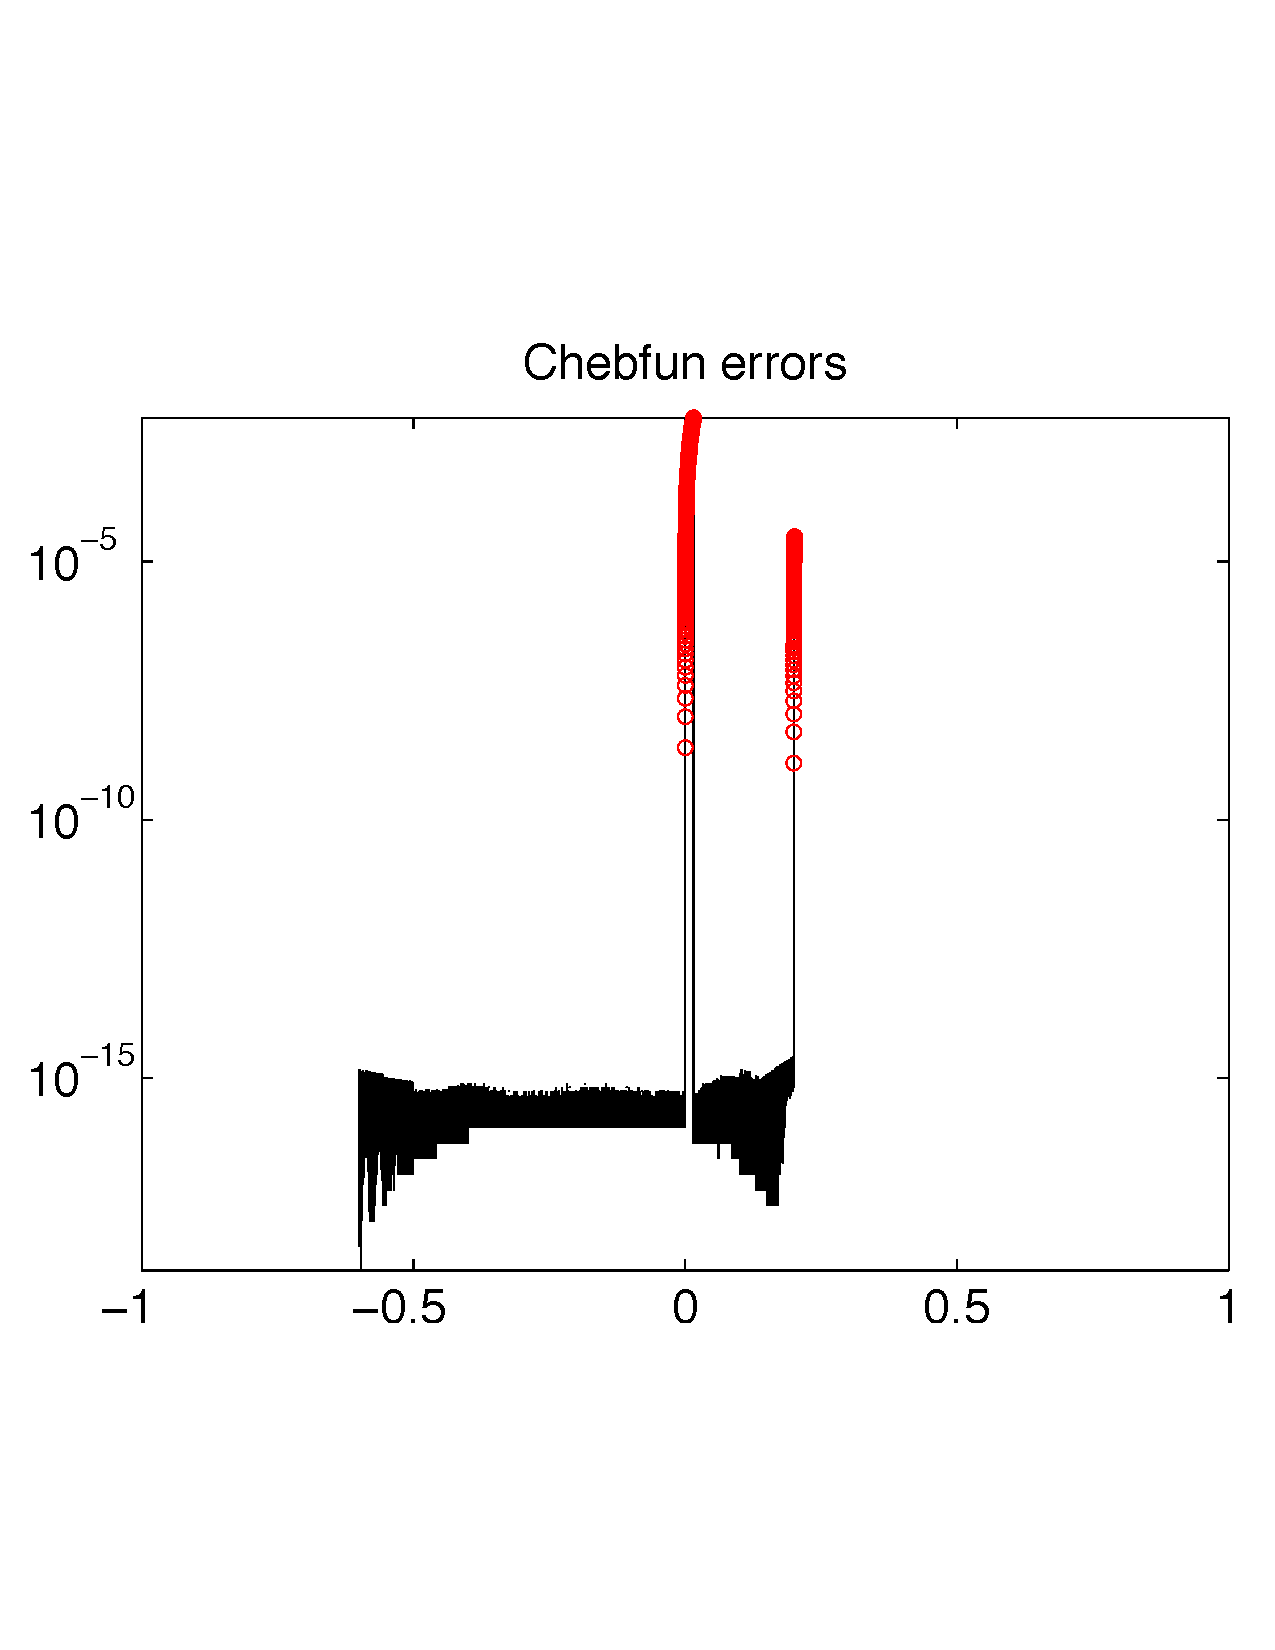
\includegraphics[width=5.9cm]{figure/chebfun_errors.pdf} \hspace{-2ex} &
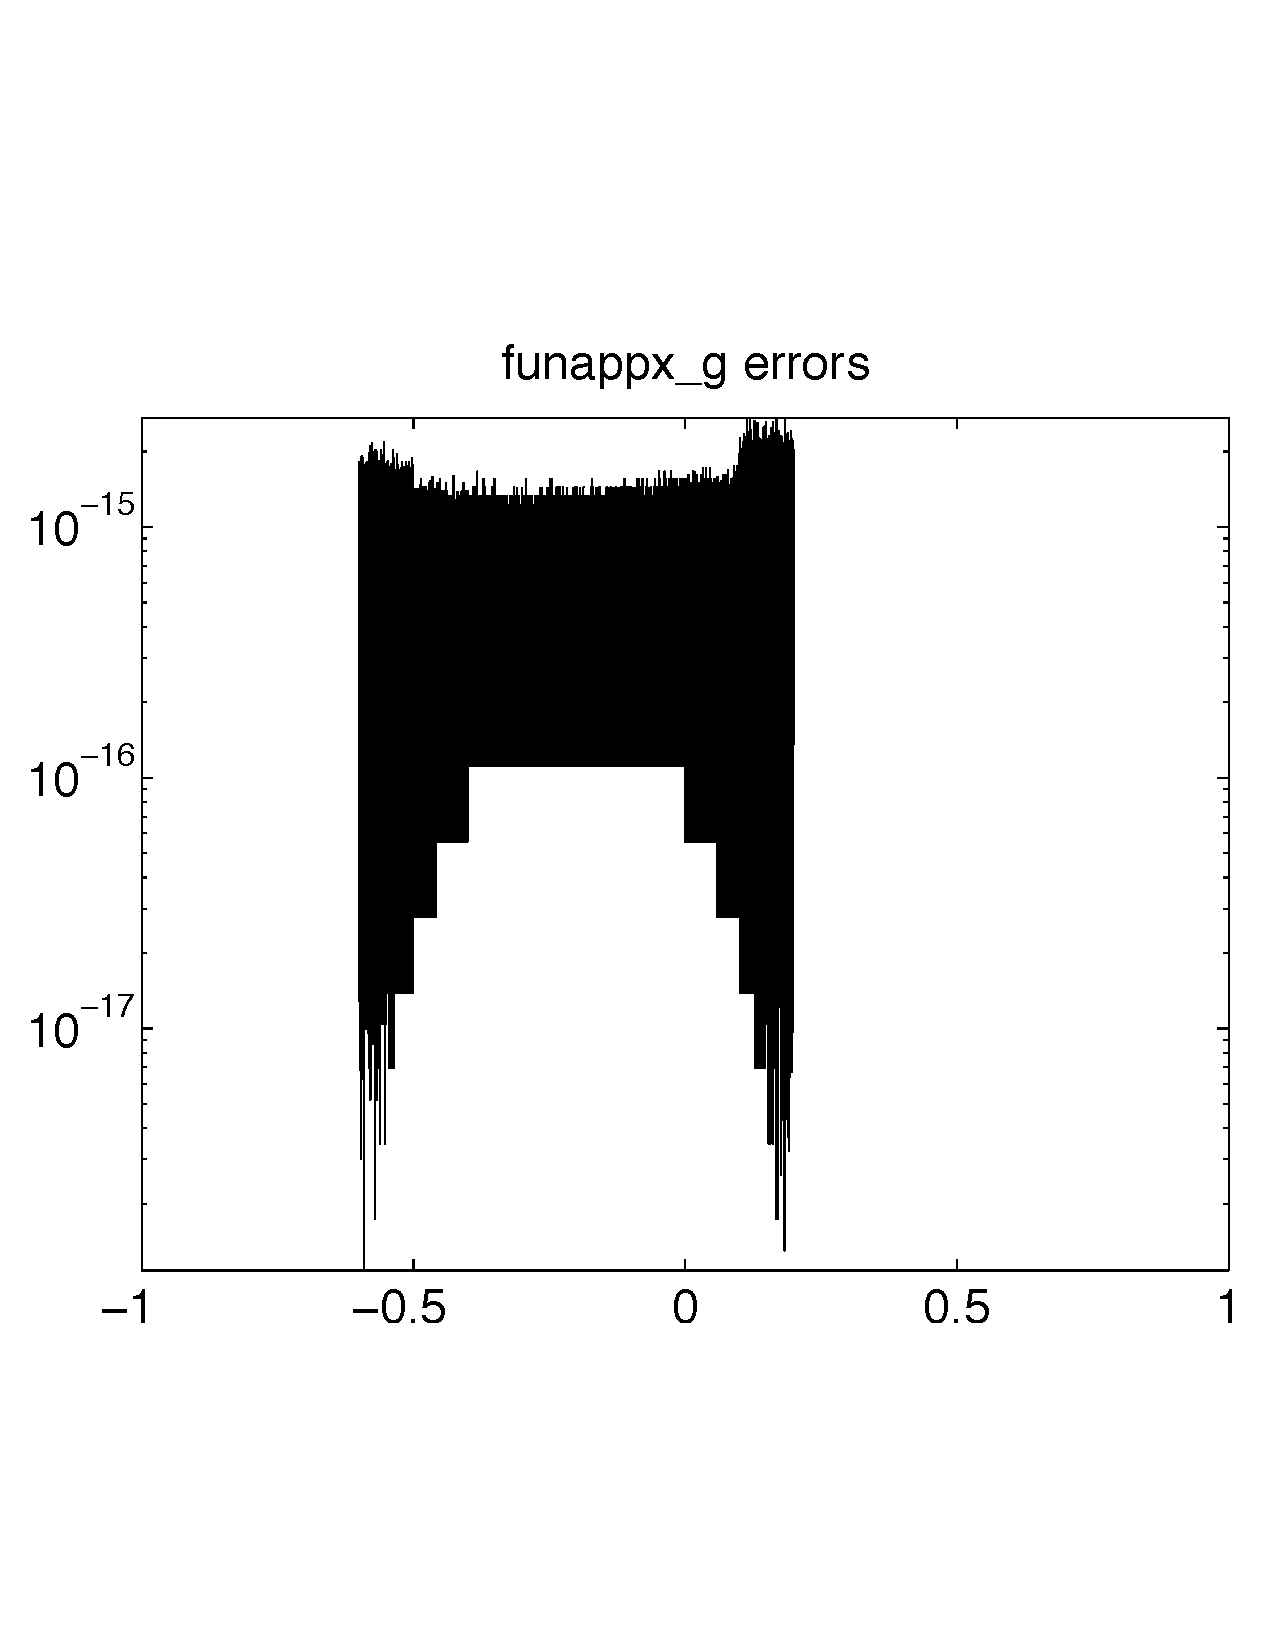
\includegraphics[width=5.9cm]{figure/funappx_g_errors.pdf}
\\ a) & b)
\end{tabular}
\caption{Approximating $f_3(x)$ with errors of interpolants returned from a)
Chebfun and b) \funappxg. This figure is reproducible by
\texttt{cf\_chebfun.m}.}
\label{f3fig}
\end{figure}
%

\end{exmp}

\begin{comment}
Our algorithm is readily extensible to the following complex-valued function.
\begin{exmp} This example is taken from MATLAB's documentation for
\texttt{interp1}. Define the complex valued function $v(x) = 5x + x^2 i$ for $x
\in [1,10]$. It is clear that the real part of $v$ is $5x$ and the imaginary
part is $x^2$. We could apply \funappxg to approximate the two parts separately.
However, it is unnecessary.
\end{exmp}
\end{comment}

%% Example 3.3

\begin{exmp}
In this example, we want to compare our adaptive algorithms with Chebfun by
simulating the following families of test functions:

\begin{align*}
 g_1(x) &= x^4 \sin(d/x), \qquad
 g_2(x) = 10  x^2 + g_1(x),
\\ g_3(x) &= \begin{cases} \displaystyle
   \frac{1}{2\delta^2} \Bigl [4 \delta^2 + (x-c)^2 + (x-c-\delta)\abs{x-c-\delta}
\\ \qquad \qquad
    - (x-c+\delta)\abs{x-c+\delta} \Bigr ], & \abs{x-c} \le 2\delta,
\\ 0, & \text{otherwise},
\end{cases} \\
 g_4(x) & = (x-d)^2, \qquad
 g_5(x)= d\sin(d\pi x), \qquad
 g_6(x)= 10\exp\left(-1000(x-d)^2\right), \qquad
% \\ f_4(x)&= \frac{c}{4}\exp(-2x)(c-2\exp(x)(-1 + c\cos(x) - c\sin(x)) \\
%  & \ \ +\exp(2x)(c + 2\cos(x)- 2\sin(x) - c\sin(2x))),
\end{align*}
where $c$ for defining $g_3$ is uniformly drawn $100$ times from $[0,0.6]$ and
$d$ for other functions from $[0,4]$. If $c=d=1$, then $g_i$ reduces to $f_i$
for $i=1,2, \mbox{and } 3$. Figure~\ref{fig:testfunctions}a) shows the shapes of
the test functions when $c=2.5$ and $d=0.375$. We set $\abstol = 10^{-6}$ and
use \texttt{funappx\_g} and \texttt{funappxglobal\_g} to approximate the test
functions on interval $[a,b]=[0,1]$ for $g_1,g_2, \mbox{and } g_3$ and
$[a,b]=[a,c+1]$ for $g_4,g_5, \mbox{and } g_6$. We summarize the approximation
results in Table~\ref{tab:localVsGlobalVsChebfun}, in which we can see that the
locally adaptive method save computational cost compared to the globally
adaptive method in all cases.

%
\begin{figure}[th]
  \centering
  \begin{tabular}{cc}
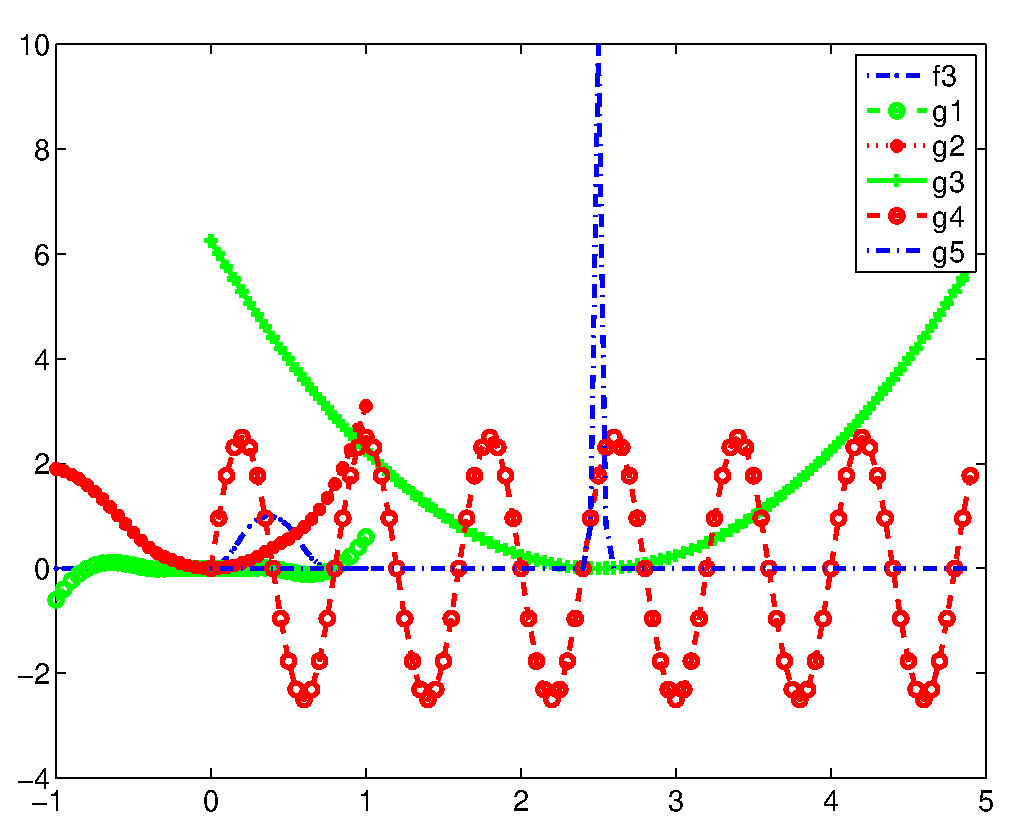
\includegraphics[width=59mm]{figure/traub_funappxNoPenalty_g_testfun.eps} & \hspace{-3ex}
\includegraphics[width=60mm]{figure/traub_funappxNoPenalty_g_test}
  \\ a)  & b) 
  \end{tabular}
\caption{a) Test functions for comparing \funappxg, \funappxglobalg, and
Chebfun. b)  Ratios of run time and number of nodes used by \funappxg{} to \funappxglobalg{} (LEFT)
to Chebfun (RIGHT). This figure is conditionally reproduced by
\texttt{traubpaper\_funappx\_g\_test.m}.}
  \label{fig:testfunctions}
\end{figure}

%
\begin{table}[bth]
\centering
\caption{Comparison of number of sample points, computational time, success and
failure rates of \funappxg, \funappxglobalg, and
Chebfun. We also report the number of warnings in parentheses issued by the
sofwtare. This table can be conditionally reproduced by
\texttt{traubpaper\_funappx\_g\_test.m}.}
\label{tab:localVsGlobalVsChebfun}
{\footnotesize
\setlength{\tabcolsep}{.2em} % set table width
\begin{tabular}{|c|rrr|rrr|rrrrrr|rr|}
\hline
    Test      &     \multicolumn{3}{c|}{Number of Points} & \multicolumn{3}{c|}{Time Used}  & \multicolumn{6}{|c|}{Success} &  \multicolumn{2}{c|}{Failure}
\\  functions &  Local  &  Global    &  Chebfun & Local       &  Global  & Chebfun              & \multicolumn{2}{c}{Local}   &  \multicolumn{2}{c}{Global}  & \multicolumn{2}{c}{Chebfun}  & \multicolumn{2}{|c|}{Chebfun}  
\\ \hline
      $g_1$ &   4152  &   30357  & 5069   &   0.052   &  0.030  &  3.989  &    100  & (100) &  100  &  (0) &     61 &   (24)  &    39  &  (39) 
\\    $g_2$ &   4223  &   51050  & 4720   &   0.057   &  0.038  &  3.563  &    100  & ( 72) &  100  &  (0) &    100 &   (51)  &     0  &  ( 0) 
\\    $g_3$ &    867  &   14640  &    4   &   0.046   &  0.014  &  0.094  &    100  & ( 34) &  100  &  (0) &     96 &   ( 0)  &     4  &  ( 0) 
\\    $g_4$ &   5011  &   46049  &    3   &   0.026   &  0.029  &  0.011  &    100  & (100) &  100  &  (0) &    100 &   ( 0)  &     0  &  ( 0) 
\\    $g_5$ &  29671  &  110027  &   37   &   0.059   &  0.032  &  0.016  &    100  & (  0) &  100  &  (0) &    100 &   ( 0)  &     0  &  ( 0) 
\\    $g_6$ &  11580  &  509263  &  127   &   0.037   &  0.138  &  0.129  &    100  & (100) &  100  &  (0) &     82 &   ( 0)  &    18  &  ( 0) 
\\ \hline
\end{tabular}
}
\end{table}
%

From Table~\ref{tab:localVsGlobalVsChebfun}, we see that both \funappxg{} and
\funappxglobalg{} achieved total success. The former worked better than
\funappxglobalg{} for all test cases in terms of \emph{average} number of run
time and number of sampling points. It was also more \emph{cautionary} since it
issued more warnings than \funappxglobalg.
%
In contrast, Chebfun generally used substantially less number of node points
than \funappxg{} even though the run time was not shorter in about~30\% of the
test cases; see Figure~\ref{fig:testfunctions}b)(RIGHT). However it was
particularly challenged by the highly oscillatory functions $g_1$ and $g_2$ in
terms of run time and success rates. In some instances of the peaky functions
$g_3$ and $g_6$, it failed to approximate them satisfactorily for about~10\% of
the cases.
\end{exmp} 

\begin{comment}
\begin{exmp}
In this example, we consider the function $f_4(x) = sin(10 \pi x^4) + x$, which
is increasing oscillating over the interval $[0,2]$. We use \funappxg, \funming,
and \integralg to approximate the function, locate its global minimum, and
estimate its integral with $\abstol = 10^{-8}$. With $1,972,359$ points,
\funappxg can approximate $f_4$ uniformly accurate as shown in
Figure~\ref{f4fig}(a). The true global minimum is $(0.6212340312,
-0.3782149854)$ and the absolute approximation error of \funming using
$n=2,022,621$ points is $(1.4\times 10^{-7}, 4.7\times 10^{-11})$. The integral
$\int_{0}^{2} f_4 (x) dx = 2.145517314$ and the approximation error of
\integralg is $4.7\times10^{-10}$ using $4,965,641$ points.

\begin{figure}[bt]
\centering
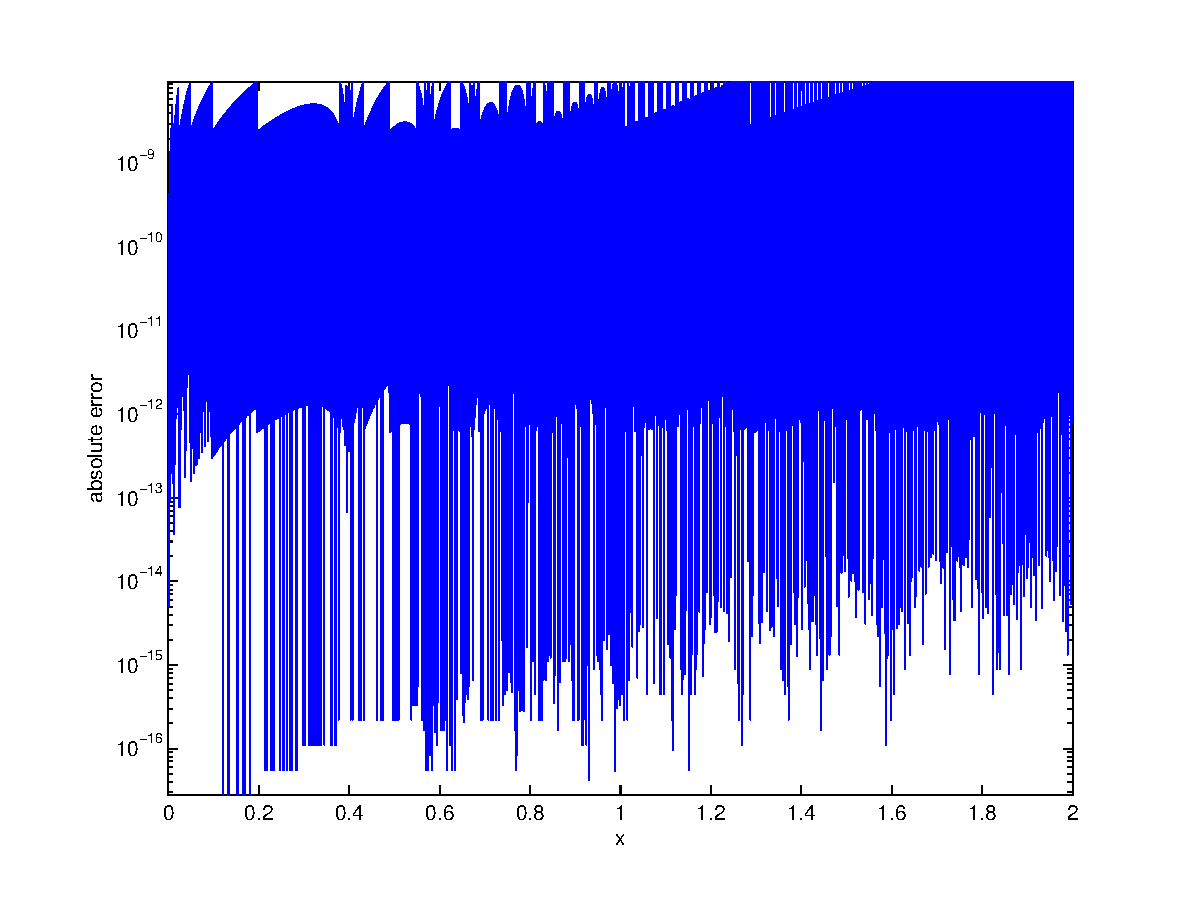
\includegraphics[width=6.2cm]{figure/f4_funappx_error.eps} \hspace{-5ex}
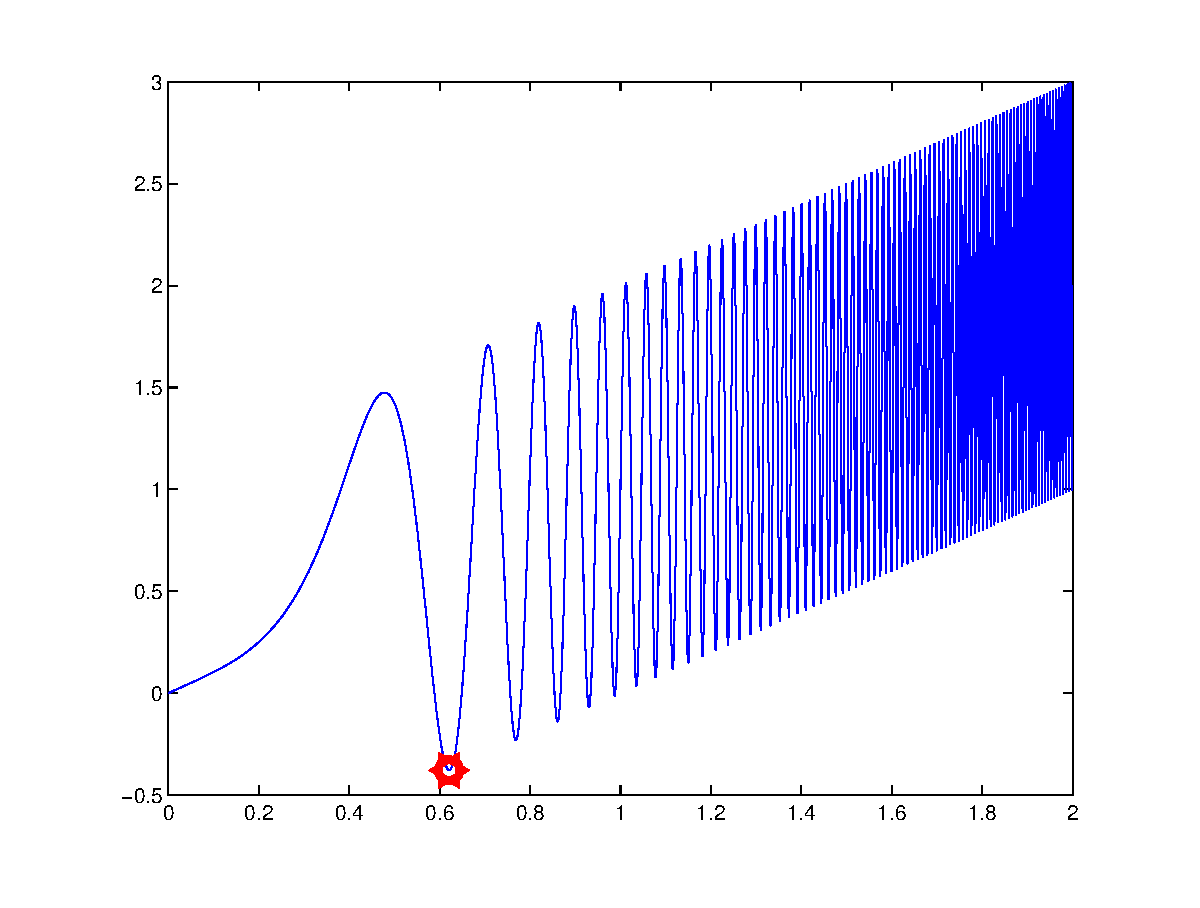
\includegraphics[width=6.2cm]{figure/f4_funmin_g.eps}
\caption{The example $f_4$ with errors of interpolants from \funappxg (left) and
minimum found by \funming (right).}
\label{f4fig}
\end{figure}
\end{exmp}
\end{comment}


     
\begin{comment}
Our algorithm is readily extensible to the following complex-valued function.
\begin{exmp}
This example is taken from MATLAB's documentation for \texttt{interp1}. Define
the complex valued function $v(x) = 5x + x^2 i$ for $x \in [1,10]$. It is clear
that the real part of $v$ is $5x$ and the imaginary part is $x^2$. We could
apply \funappxg to approximate the two parts separately. However, it is
unnecessary.
\end{exmp}
\end{comment}

 



\section{Discussion}


%%%%%%%%%%%%%%%%%%%%%%%%%%%%%%%%%%%%%%%%%%%%%%%%%%
\section*{References}
%%%%%%%%%%%%%%%%%%%%%%%%%%%%%%%%%%%%%%%%%%%%%%%%%%

\bibliography{FJH23,FJHOwn23}

\end{document}








